\documentclass{ifri}
\usepackage{titletoc}
\usepackage{fancyhdr}
\usepackage{makecell}
\usepackage{enumitem}
\usepackage{minted}
\usepackage[backend=biber]{biblatex}

\addbibresource{bibliography.bib}
\graphicspath{ {./images/}}
\setlength{\arrayrulewidth}{0.5mm}
\setlength{\tabcolsep}{5pt}
\renewcommand{\arraystretch}{1.5}
\renewcommand\theadalign{bc}
\renewcommand\theadfont{\bfseries}
\renewcommand\theadgape{\Gape[4pt]}
\renewcommand\cellgape{\Gape[4pt]}

\renewcaptionname{english}{\listfigurename}{Liste des Figures}
\renewcaptionname{english}{\listtablename}{Liste des Tables}

\setlength{\glsdescwidth}{0.65\textwidth}

\typeMemoire{Diplôme de Licence en Informatique}
\optionFormation{Génie Logiciel}
\etudiant{Hans Bignon. K. \textbf{TOGNON}}
\titreDuMemoire{Conception d'un SaaS pour les cours en ligne en milieu universitaire}

\dateSoutenance{-}
%\promo{2\up{ème}}
% \anneeScolaire{2021-2022}


%%maitre de mémoire
% \encadrants{Ing. Miranda \textbf{GNONLONFOUN}}


\hypersetup{
pdftitle={Conception d'un SaaS pour les cours en ligne en milieu universitaire},
pdfauthor={Hans TOGNON},
pdfsubject={--},
pdfkeywords={Sass, Studx, WebRTC, online classes}
}

\color{bookColor}

%importation du glossaire
\loadglsentries{glossaire}

\begin{document}


\pagecolor{white}

%% page vide
%\thispagestyle{empty}\ \clearpage


\selectlanguage{french}

% sommaire
\pagenumbering{roman}

% \setcounter{tocdepth}{0}
% \startlist{toc}
% \printlist{toc}{}{\chapter*{Sommaire}}
% \setcounter{tocdepth}{5}

% Résume
\resume
\selectlanguage{french}
\vspace*{-6cm}
\begin{abstract}
L'enseignement supérieur doit s'adapter aux nouvelles contraintes que l'on observe aujourd'hui comme l'incapacité
d'assiter aux cours presentiels en raison de facteurs comme les pandémies. Les technologies de communication en temps
réel offrent une bonne alternative qui revient d'exploiter. Dans le but de favoriser l'emploi de ces outils de communication,
nous proposons StudX, un prototype d'application permettant la tenue de classes virtuelles. Le processus de 
développement de cette plateforme a requis l'emploi de techniques modernes de modélisation logicielle, de technologies de pointe et de ressources appropriées.

\paragraph{}
\textbf{Mots clés}: StudX,WebRTC,cours en ligne,universités,communication en temps réel
\end{abstract}

\newpage
\thispagestyle{empty}
\selectlanguage{english}
\addcontentsline{toc}{chapter}{Abstract}
\begin{abstract}

Higher education must adapt to the new constraints that we observe today such as the inability to attend
to attend face-to-face classes due to factors such as pandemics. Real-time communication technologies offer a good alternative
technologies offer a good alternative that is worth exploiting. In order to promote the use of these communication tools
we propose StudX, a prototype application for virtual classes. The development process of this 
The development process of this platform required the use of modern software modeling techniques, state-of-the-art technologies and appropriate resources.

\paragraph{}
\textbf{Key words}: StudX,WebRTC,online classes,universities,real time communication
\end{abstract}
\newpage

%liste des figures
% \listoffigures{Liste des figures} 
% \newpage

% %liste des tableaux
% \listoftables{Liste des tableaux}
% \newpage

%liste des algo
% \selectlanguage{french}
% \newpage

% % Les sigles et acronymes
% \setglossarystyle{altlist}
% \printnoidxglossary[title=Liste des acronymes, toctitle=Liste des acronymes, type=\acronymtype]
% \newpage

% % Le glossaire proprement dit
% \setglossarystyle{super}
% \printnoidxglossary[type=main]


\pagenumbering{arabic}
\setcounter{page}{1}
%%introduction

\introduction

\thispagestyle{plain} % removes unneeded heading

% TODO: Add a small corpus before the texts below

\section*{Contexte}
Les temps changent et les méthodes d’enseignement également. 
Dans le cadre de la mondialisation, on assiste à l'emploi du numérique, 
avec des méthodes de plus en plus créatives et collaboratives, 
pour une meilleure éducation. Cela reste valable dans le milieu de l’enseignement supérieur.
Il va sans dire que des facteurs comme la pandémie de COVID-19 ou encore, 
l'indisponibilité de cadres de cours adéquats, 
rendent plus urgent le besoin de transitionner 
vers des salles de classe virtuelle, pour répondre aux besoins. 
De ce fait, les technologies de l’information et 
de la communication constituent un atout décisif dans le succès de cette transition.

\section*{Problématique}
L’expansion des cours en ligne est désormais un fait. 
Cela requiert une organisation logistique accrue et un investissement financier pour les entités universitaires. 
Toutefois, l’on note l’emploi de solutions génériques, qui rendent difficile, 
voire impossible l'émulation d’un environnement de classe. 
Pour peu qu’elles soient conformes aux exigences, c’est alors le prix qui peut poser problème. 
C’est la raison d'être de notre projet, qui vise la mise en place d’une application, 
pour répondre au besoin d'interactivité lors des cours en ligne, 
et éliminer les barrières d’ordre logistique et financier, imposées par les solutions génériques.

\section*{Objectifs}
Le principal objectif est la conception de StudX, un prototype d’application SaaS, permettant la tenue de cours en ligne.
En termes de fonctionnalités et buts, il s’agira notamment de pouvoir :
\begin{itemize}
  \item organiser les différentes classes, filières ou promotions des entités en sections bien définies ;
  \item définir le calendrier des cours à tenir ;
  \item organiser des sessions d’audio-conférence pour le déroulement des cours ;
  \item mettre en place des fonctionnalités telles le partage d'écran et bien d’autre pour émuler un tant soit peu, 
    un environnement de classe présentiel ;
  \item minimiser les coûts requis dans le cadre de la mise en oeuvre d’une solution de classe virtuelle.
\end{itemize}

\thispagestyle{plain} % removes unneeded heading

\section*{Organisation du document}
Le présent document renferme trois chapitres. 
Dans le premier chapitre, nous ferons une revue de littérature sur le sujet 
et présenterons les généralités sur quelques notions essentielles. 
Le second chapitre relate les méthodes employées pour la conception de notre solution ainsi 
que les outils et matériels utilisés à cette fin. 
Le dernier chapitre sera consacré à la présentation des résultats obtenus, 
des interfaces conçues ainsi que des potentielles insuffisances liées à la solution que nous avons développée.

%\lhead[]{} \rhead[]{} \chead[]{}
\selectlanguage{french}
\fancyhead[L]{\tiny \leftmark}
\fancyhead[R]{\scriptsize \rightmark}
\fancyfoot[C]{\thepage}

\chapter{Revue de littérature}\label{chap:1}
\addcontentsline{toc}{section}{Introduction}
\section*{Introduction}

Le concept de la formation à distance ne date pas d’hier. 
Dans ce chapitre, nous ferons une revue des origines de cette méthode d’enseignement. 
S’en suivra une analyse des techniques modernes de communication en temps réel et des solutions existantes qui permettent  de dispenser des cours à distance.

\section{Formation à distance}

L'encyclopédie Wikipedia définit la formation à distance comme une 
forme d’enseignement ou l’enseignant et l'étudiant sont séparés 
dans le temps et/ou par l’espace \cite{distance_education}.

\subsection{Origines}

Les premiers essais de formation à distance remontent à bien avant l'ère moderne. 
En effet, déjà en 1728, Caleb Phillips, un professeur, 
recherchaient des étudiants désirant acquérir des compétences en sténographie, 
auxquels il dispensait les cours par courrier.

Au sens moderne, le premier cours d’enseignement à distance, est attribué à Isaac Pitman, toujours en rapport avec la sténographie. 
Un nouvel élément qui apparaît dans le cas actuel, c’est la rétroaction des étudiants, 
qui devaient envoyer leurs transcriptions par la poste, pour correction. 
Ce mode de fonctionnement fut rendu possible par l’uniformisation des tarifs postaux en Angleterre. 
Plusieurs institutions telles que Oxford et l'université de Londre ont également expérimenté l’enseignement à distance.

Aujourd’hui, l’expansion d’Internet et du World Wide Web, permettent la mise en œuvre des moyens toujours plus sophistiqués, pour dispenser les cours à distance.


\subsection{Internet et formations en ligne}

L'avènement des nouvelles technologies de l’information et de la communication 
a donné lieu à la mise en place des formations en ligne, 
une forme évoluée de formation à distance \cite{online_learning}. 
En 2020, par exemple, sous l’impulsion de la pandémie alors en cours, 
plusieurs universités dont celle d’Abomey-Calavi, 
effectuent la transition partielle ou totale vers les classes virtuelles \cite{etudiant_dot_bj}.

On distingue deux environnements d’apprentissage. 
D’une part, les environnements asynchrones, qui offrent une totale liberté à l'apprenant quant à la gestion de son temps. 
L’enseignant et lui sont séparés littéralement par le temps et la distance. Ainsi, il peut consulter les ressources au moment qui lui convient le mieux. 
Cela permet une assimilation plus facile, étant donné que chaque apprenant peut s’adapter en fonction de ses besoins spécifiques. 
Toutefois, il est possible que l’apprenant se retrouve isolé et ne fasse finalement aucun progrès, faute de support.

D’autre part, un environnement synchrone essaie d'émuler une classe présentiel, 
à la seule différence que les participants sont physiquement distants. 
Avec des outils de messagerie instantanée et/ou de visioconférence, 
les apprenants peuvent interagir avec leurs pairs ainsi que le ou les enseignants.

En termes de classification des diverses formes de cours en ligne, Andreas Kaplan, 
auteur du livre \textit{Contemporary Issues in Social Media Marketing} \cite{andreas_kaplan_classfication}, propose une approche simplifiée basée sur les facteurs 
comme le temps, la distance et le nombre d’apprenants. 
Le tableau ci-dessous, en fait un récapitulatif.

% \begin{table}[]
%   \begin{tabular}{lllll}
%    &  &  &  &  \\
%    &  &  &  &  \\
%    &  &  &  &  \\
%    &  &  &  & 
%   \end{tabular}
% \end{table}

Notons que notre étude s'intéresse notamment aux environnements d’apprentissage synchrones, 
avec le support d’un grand nombre d’apprenants, ce qui correspond bien aux SMOCs.

\section{Communication en temps réel}
Les outils de communications en temps réel désignent une catégorie de logiciels qui garantissent le traitement et la transmission instantanée, 
ou avec un délai fortement négligeable,  de l’information. 
Parmi les protocoles permettant ce type de communication, le plus en vogue reste WebRTC.


WebRTC est un protocole open source de transmission P2P, qui assure la transmission de média (audio, vidéo) 
et de données brutes, presque sans latence (moins d’une seconde), 
le tout dans un contexte hautement sécurisé. 
Il s’agit en réalité, d’une collection de protocoles datant des années 2000 [ref webrtcforthecurious]. 
Pour établir une connexion, il faut quatre étapes à savoir la signalisation, la connexion proprement dite, la sécurisation puis la communication.

La signalisation désigne le processus initial de mise en relation des pairs. 
Sans ce processus, une machine quelconque n’a aucune idée de qui voudrait bien la contacter. 
Pour ce faire, le protocole SDP est utilisé et permet la transmission d’informations capitales comme:

\begin{itemize}
  \item l’IP et le port de chaque agent WebRTC (plusieurs variantes, en réalité)
  \item les codecs multimédia supportés
  \item d’autres valeurs comme des certificats de sécurité nécessaires à la mise en place de la connexion et la sécurisation.
\end{itemize}


A la connexion, les agents WebRTC établissent un lien direct entre eux, sans intermédiaire. 
Face à la multitude de possibilités de connexion (couples constitués de l’IP et du port), 
le protocole ICE permet de choisir le meilleur candidat, en faisant recours au serveur STUN et parfois, au serveur TURN. 
Le serveur TURN permet la retransmission des données lorsqu’il est impossible pour un agent WebRTC d'établir un lien 
direct avec un autre agent en raison de la configuration réseau (NAT et les types de liaisons possibles) [webrtc for the curious types of link].

Pour assurer la sécurité de la connexion, les protocoles DTLS et SRTP offrent une couche de chiffrement 
pour les contenus multimédia et les paquets brutes.

Enfin, les agents peuvent s'échanger de la donnée, du contenu multimédia, presque sans latence, grâce au protocoles RTP et SCTP.

WebRTC est une technologie complexe qui requiert une certaine expertise quant à la connaissance des protocoles, 
leur utilisation et la mise en œuvre d'applications en temps réel. 
Elle sert de base aujourd’hui,  la plupart des applications de communication en temps réel.

\section{Software as a Service}
Parmi les modèles de distribution de logiciels, le SaaS représente une méthode ou le concepteur ou l'entité tenant l’application, 
l'héberge en ligne et la rend accessible à ses utilisateurs. 
En terme de commercialisation, il est possible d’offrir un accès à la plateforme moyennant un abonnement ou 
l’achat d’une version privée pour les besoins des corporations.

\section{Présentation de solutions existantes}
Plusieurs solutions s’inscrivent déjà dans le cadre du déroulement de cours en ligne en temps réel. 
Nous avons choisi quelques unes à passer en revue.

Il est important de préciser que les insuffisances relevées par rapport à ces outils ne sont aucunement d’ordre technique. 
Nous nous intéressons plutôt aux aspects logistique et financier. 
En effet, un des objectifs visés est de minimiser l’investissement requis pour la mise en place d’une solution de classe en ligne, 
tout en éliminant les barrières possibles.

\subsection{Google Classroom}
Google Classroom est un outil de la suite Google pour l'éducation. 
A défaut de disposer d’un module de visioconférence, il s'intègre parfaitement avec Google Meet, à cette fin. 
L’application offre une version gratuite et dispose d’une interface accessible. 
Toutefois, pour les réunions en ligne, le nombre maximum de connexions possibles se limite à 500 participants. 
Pour les entités universitaires dont l’effectif est considérable par classe, ceci pourrait présenter un désavantage. 
Grâce à la version payante néanmoins, on peut mettre en place un live stream, pour permettre d'accéder au contenu de 
la réunion sans toutefois pouvoir interagir avec les participants. 
Le modèle de souscription aussi, basé sur le nombre d’utilisateurs risque d'entraîner des frais assez élevés.

\subsection{Zoom}
Zoom est un outil de communication très performant, qui a la capacité de supporter un grand nombre d’utilisateurs. 
Il dispose de fonctionnalités très utiles pour le déroulement de cours en ligne comme le partage d'écran ou le tableau virtuel. 
Accéder à ces fonctionnalités dans le cadre d’une utilisation à grande échelle requiert une souscription et les offres de Zoom ne sont pas des plus simples. 
En effet, Zoom dispose d’un panel large de services associés et donc, sans orientation, 
il est possible de choisir une solution inadéquate en rapport avec le besoin.


\subsection{Moodle}
Moodle est un LMS Open Source populaire très connu et utilisé dans les entités de l’enseignement supérieur. 
Il peut être hébergé ou utilisé en ligne. 
Il offre un large panel de fonctionnalités et permet l'intégration de divers modules dont des modules de visio-conférence. 
BigBlueButton est une solution Open source employée à cet effet. 
La mise en place requiert toutefois, une certaine expertise et du matériel spécifique, ce qui en limiterait la portabilité.

\addcontentsline{toc}{section}{Conclusion}
\section*{Conclusion}
Ce chapitre a permis de faire une revue de l’existant et jette les bases des 
suivants en exposant les concepts clés qui seront développés. 
Les solutions suscitées conviendraient pour un usage modéré. 
Elles peuvent s'avérer coûteuses, pour peu qu’elles répondent au besoin. 
La solution que nous proposons vise à doter les organismes de l’enseignement supérieur, 
d’un moyen simple mais efficace de tenir les cours en ligne, offrant des outils d’assistance, 
tout en minimisant les coûts, que cela pourrait engendrer.


\chapter{Résultats et Discussion}\label{chap:3}
\addcontentsline{toc}{section}{Introduction}
\section*{Introduction}
Ce chapitre s'attelle à la présentation du prototype de StudX, l’application de communication en temps réel que nous proposons. 
Nous en présenterons les diverses fonctionnalités accompagnées de capture d'écran. 
Puis, au travers d’une discussion, nous en présenterons les limites, les contraintes et les possibilités d’expansion.

\section{Résultats}
\subsection{Authentification}
L'accès à l’application est subordonné à l'authentification de l’utilisateur. 
La figure \ref{fig:proto_auth} en présente l’interface. 
Elle offre la possibilité de se connecter ou de s'inscrire.

\begin{figure}[h]
  \centering
  \frame{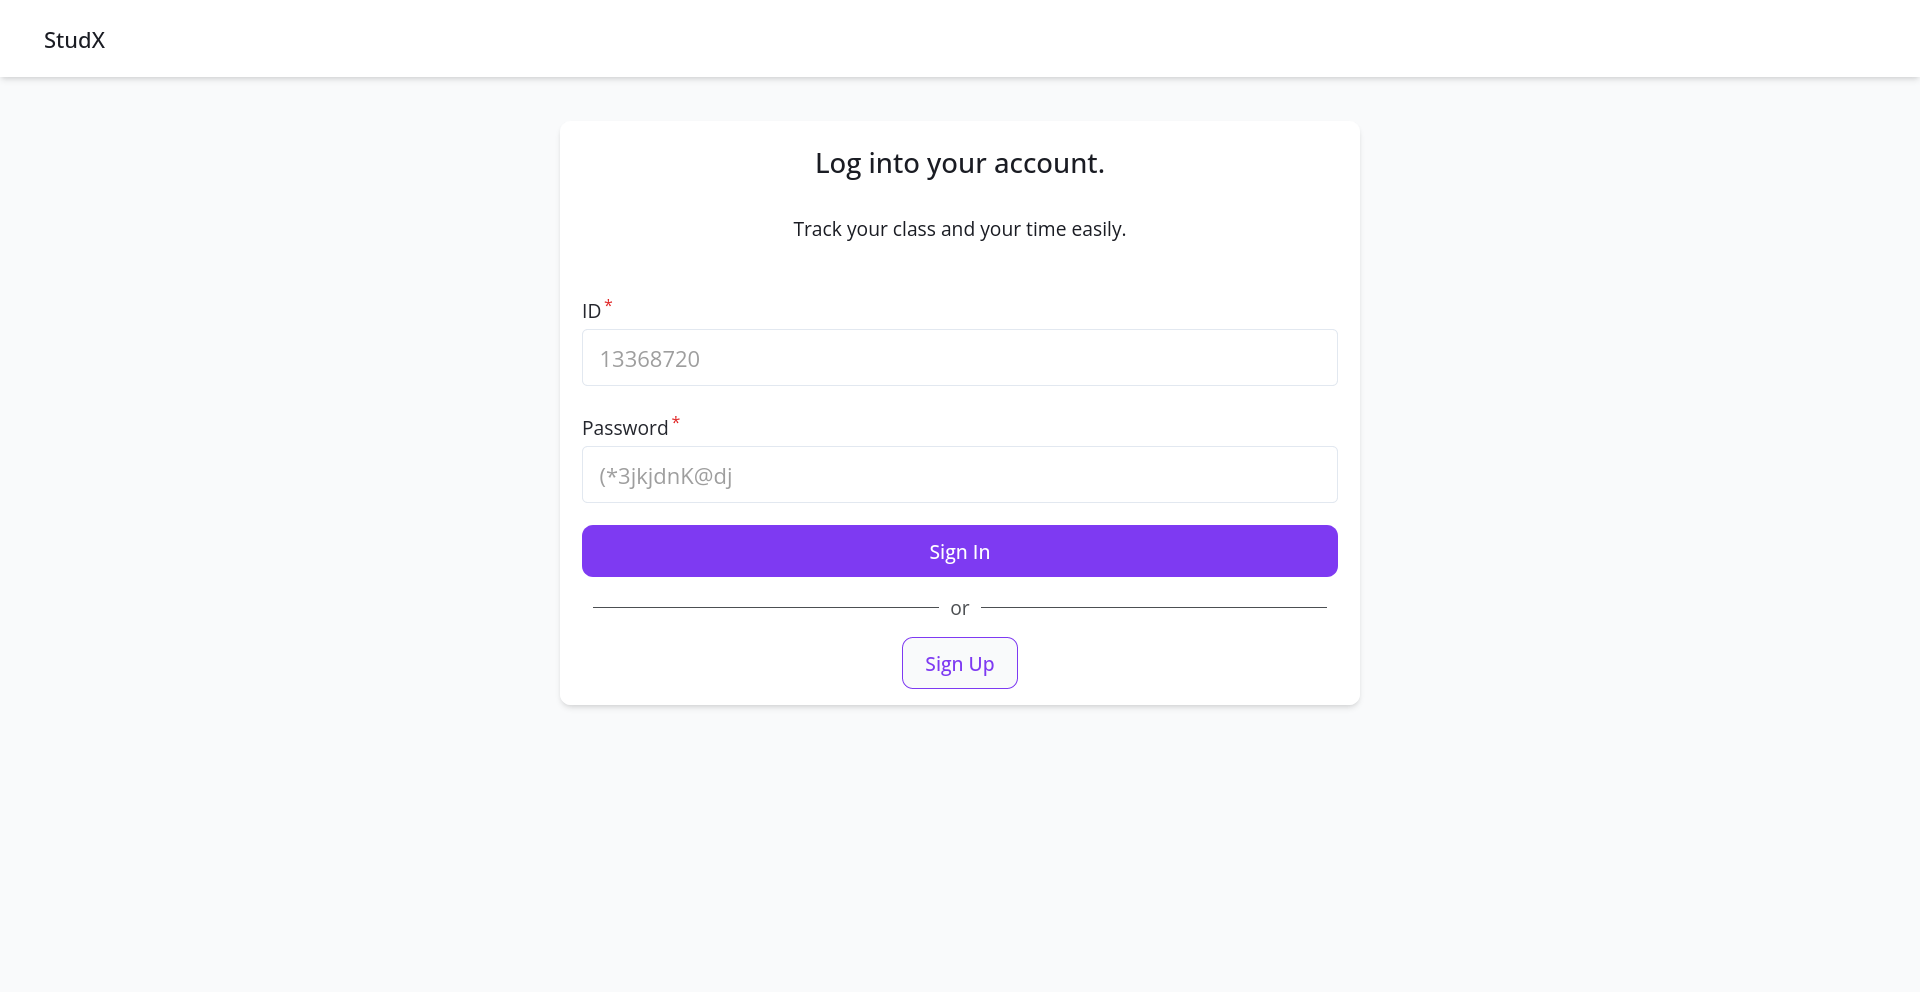
\includegraphics[width=0.85\textwidth]{prototype/login}}
  \caption{Page d'authentification de \textbf{StudX}}
  \label{fig:proto_auth}
\end{figure}

\subsection{Calendrier}
Après authentification, l’utilisateur accède au calendrier des divers événements planifiés. 
Il lui est possible de réduire ou d'étendre la vue au jour actuel, aux semaines ou encore aux mois.  
S’il s’agit d’un administrateur ou d’un enseignant, il peut en ajouter de nouveaux.
La figure \ref{fig:proto_calendar_view} présente le calendrier,qui présente tous les programmes du mois courant.

\begin{figure}[h]
  \centering
  \frame{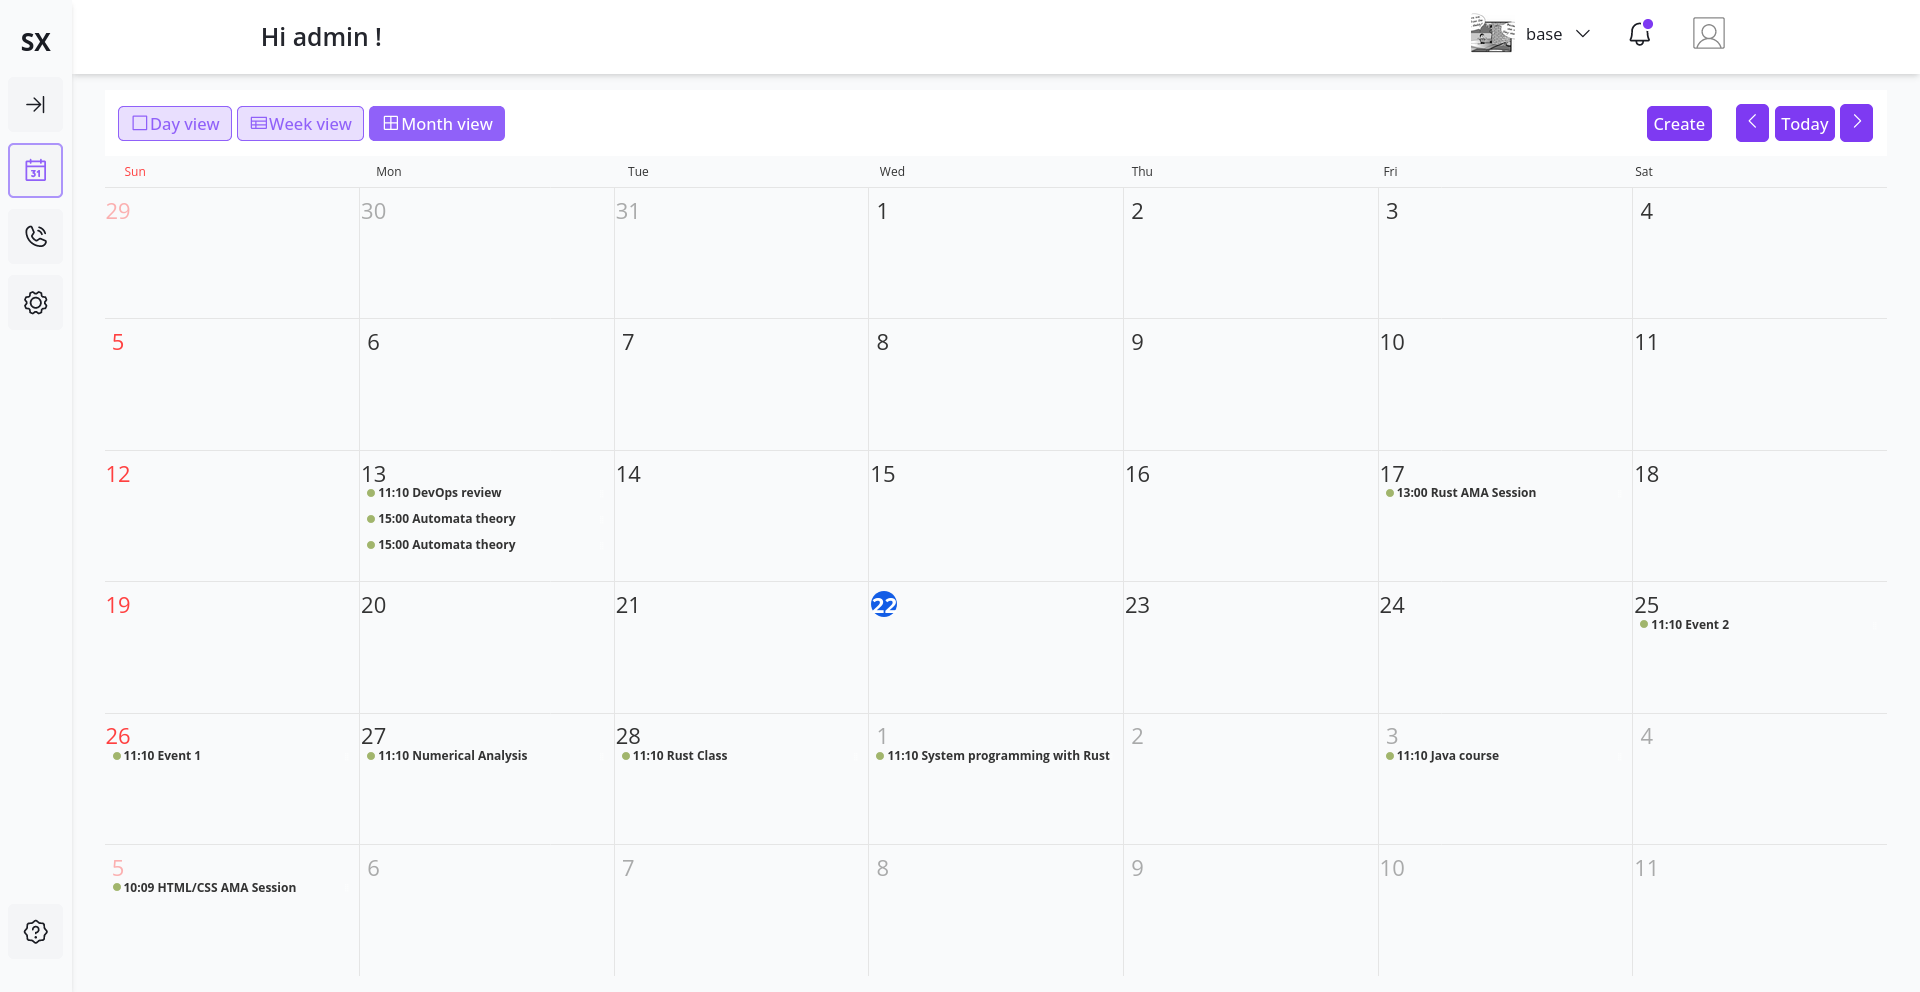
\includegraphics[width=0.85\textwidth]{prototype/calendar-view}}
  \caption{Calendrier des planifications}
  \label{fig:proto_calendar_view}
\end{figure}

S’il dispose des permissions nécessaires, 
l’utilisateur peut ajouter un événement au calendrier en suivant le formulaire que montre la figure \ref{fig:add_event}.


\begin{figure}[h]
  \centering
  \frame{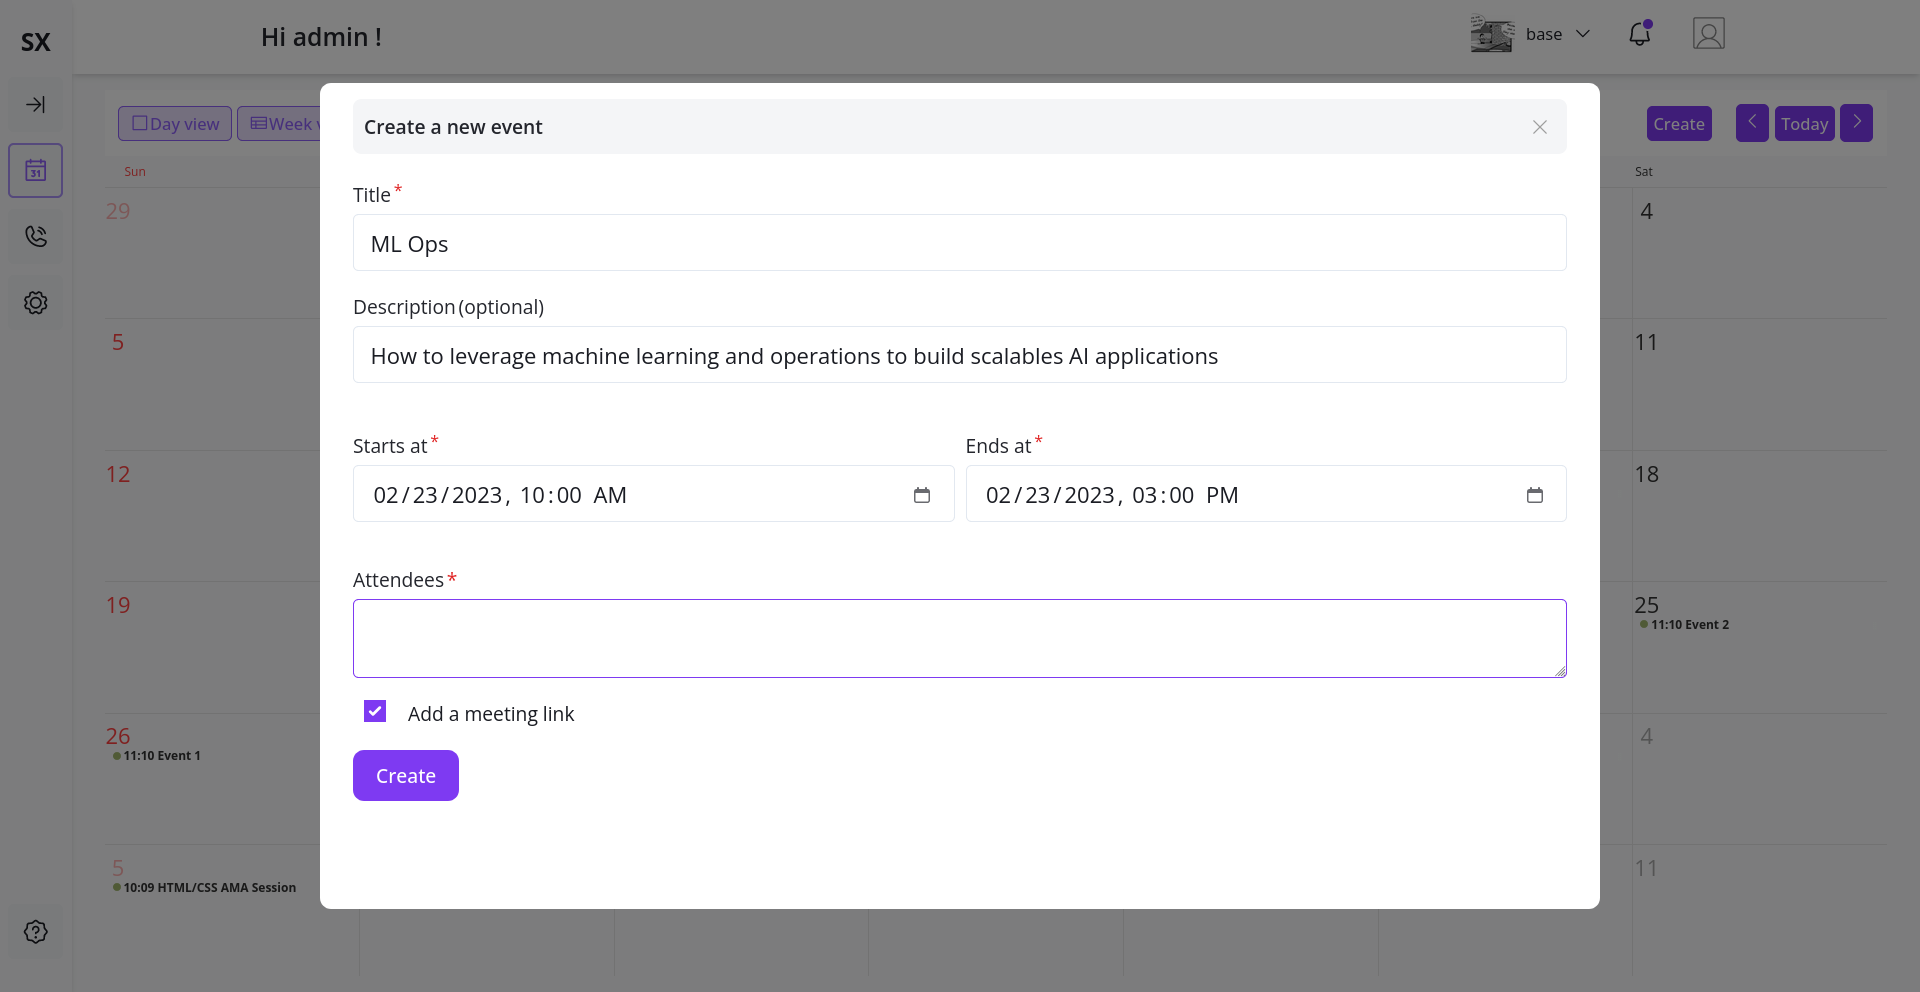
\includegraphics[width=0.85\textwidth]{prototype/add-event-form}}
  \caption{Calendrier des planifications}
  \label{fig:add_event}
\end{figure}

Il est possible d’associer à l'événement un lien d'accès à la session de conférence en ligne. 
Pour y accéder par la suite, les utilisateurs peuvent consulter les détails dudit événement (figure \ref{fig:event_details}).

\begin{figure}[h]
  \centering
  \frame{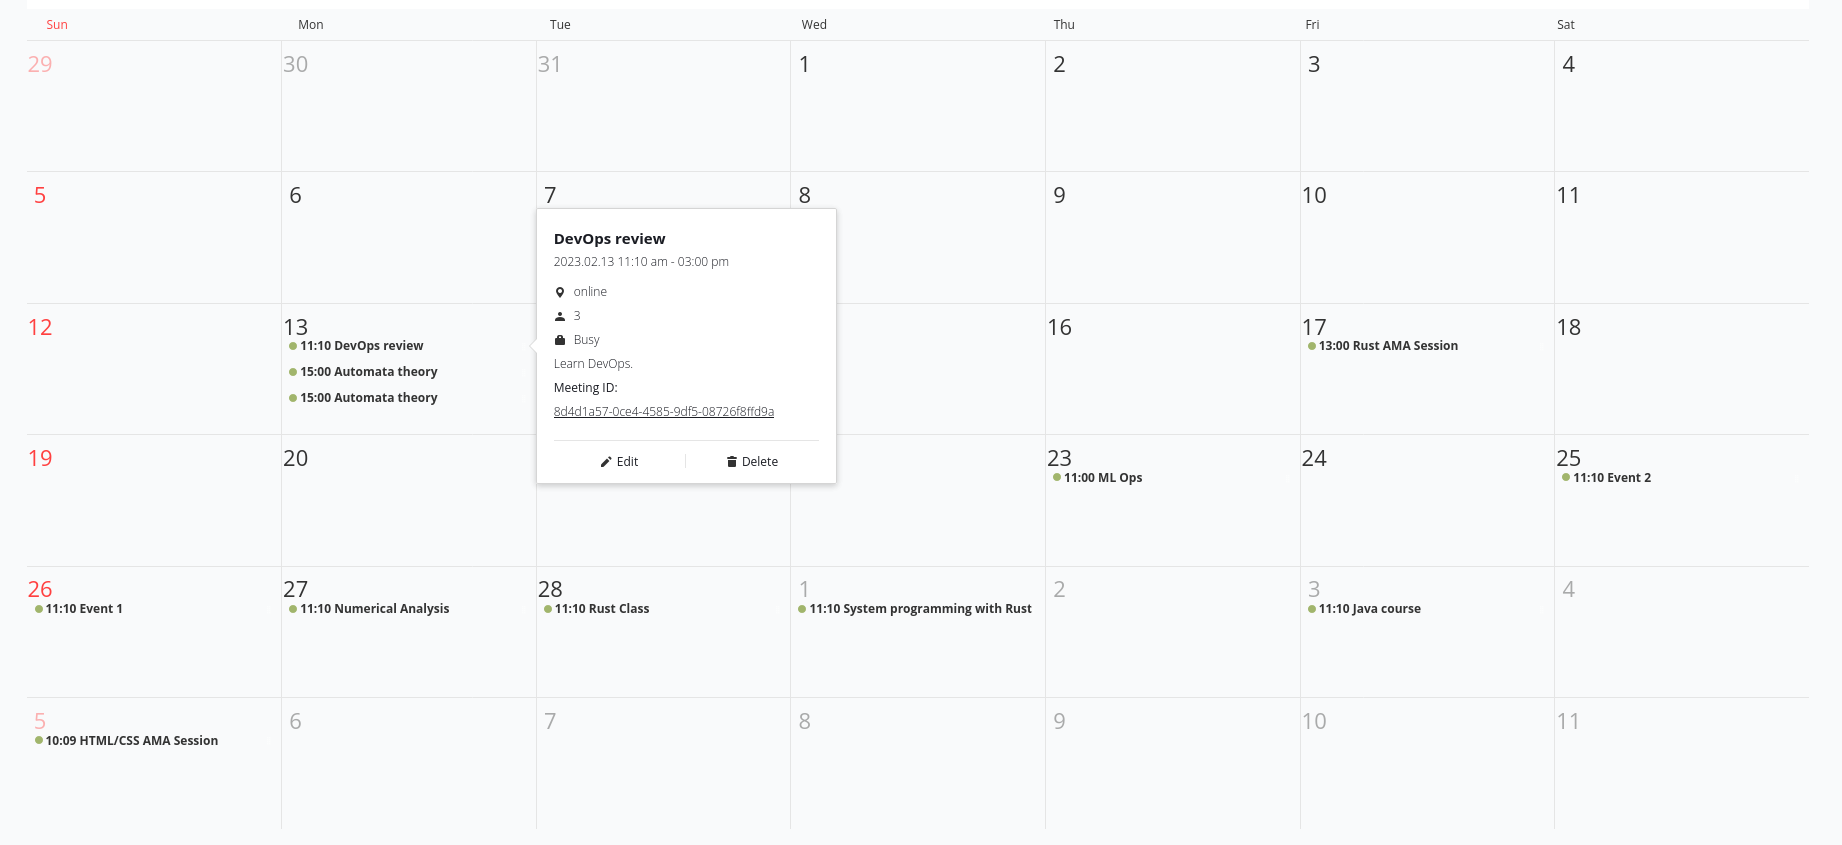
\includegraphics[width=0.85\textwidth]{prototype/event-detail}}
  \caption{Détails d'un événement}
  \label{fig:event_details}
\end{figure}

\subsection{Sessions en ligne}
Les événements incluant un lien donnent accès à une session en ligne que
peuvent rejoindre tous les participants disposant du lien.

Les figures \ref{fig:single_user} et \ref{fig:many_users} présentent à quoi ressemble l’interface par défaut. 
Elles présentent, en fait, la grille des participants et l’interface de contrôle.


\begin{figure}[h]
  \centering
  \frame{
\includegraphics[width=0.85\textwidth]{prototype/user-single-in-room}}
  \caption{Grille des participants avec un seul participant présent}
  \label{fig:single_user}
\end{figure}


\begin{figure}[h]
  \centering
  \frame{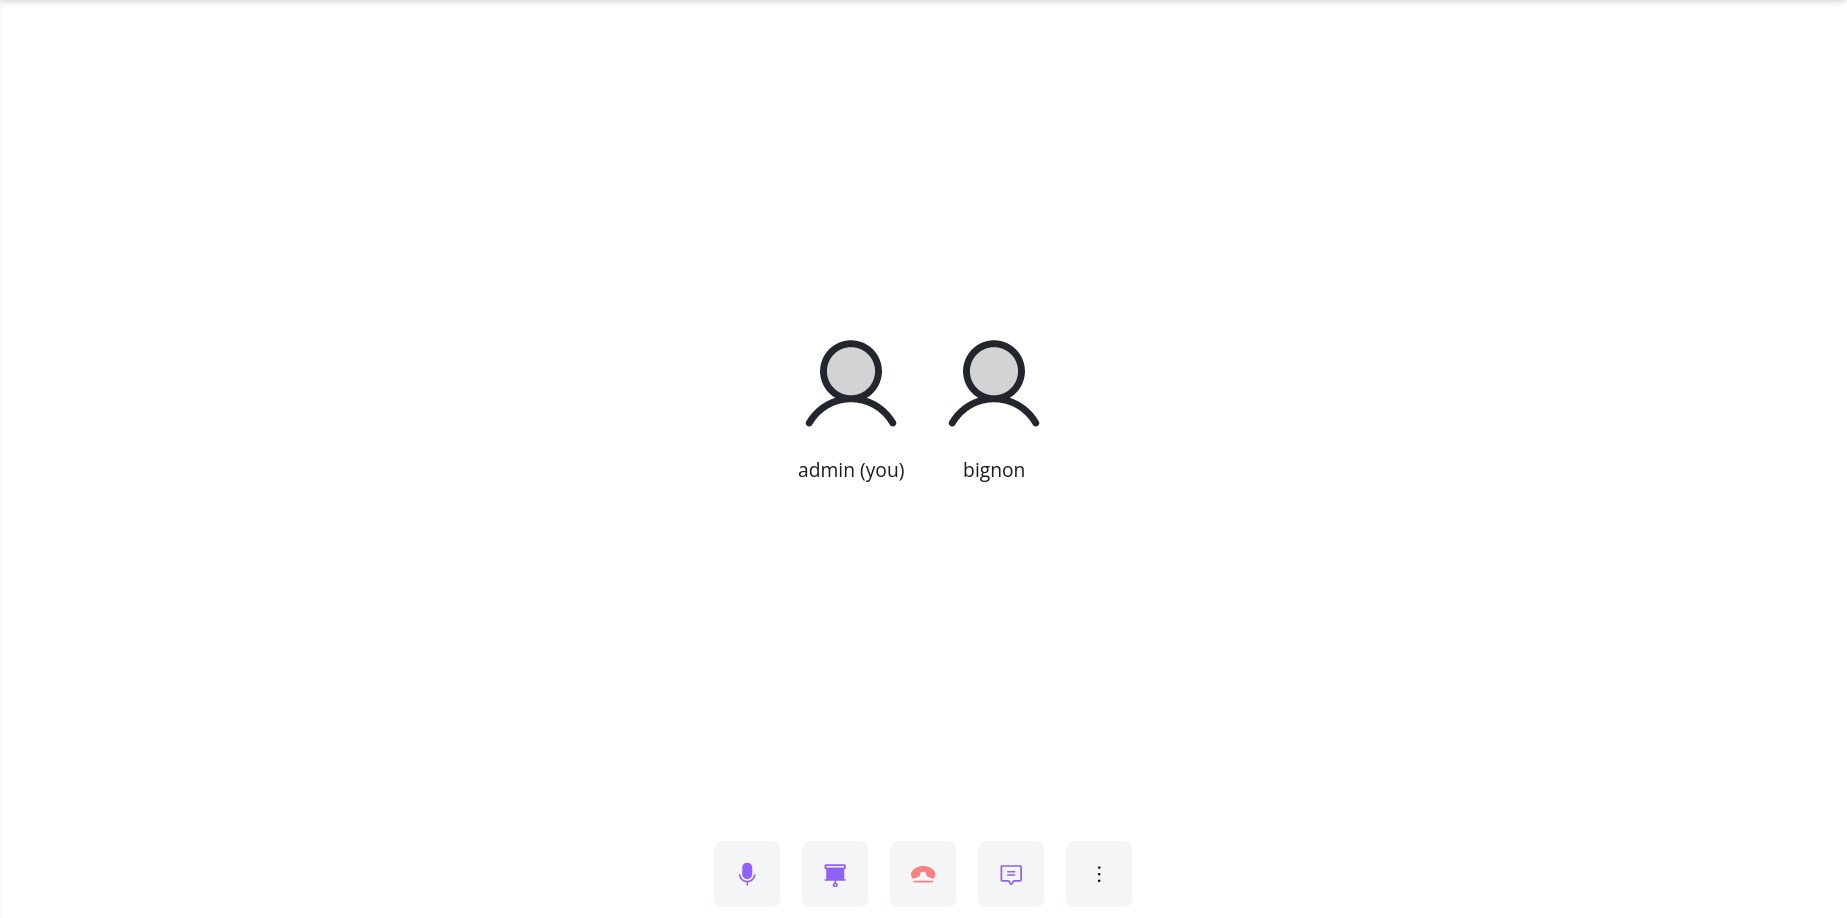
\includegraphics[width=0.85\textwidth]{prototype/user-with-participants-in-room}}
  \caption{Grille des participants avec plus d'un utilisateur}
  \label{fig:many_users}
\end{figure}

\newpage
Outre la voix, les participants ont la possibilité d’interagir entre eux via des messages écrits (figure \ref{fig:room_chat}).

\begin{figure}[h]
  \centering
  \frame{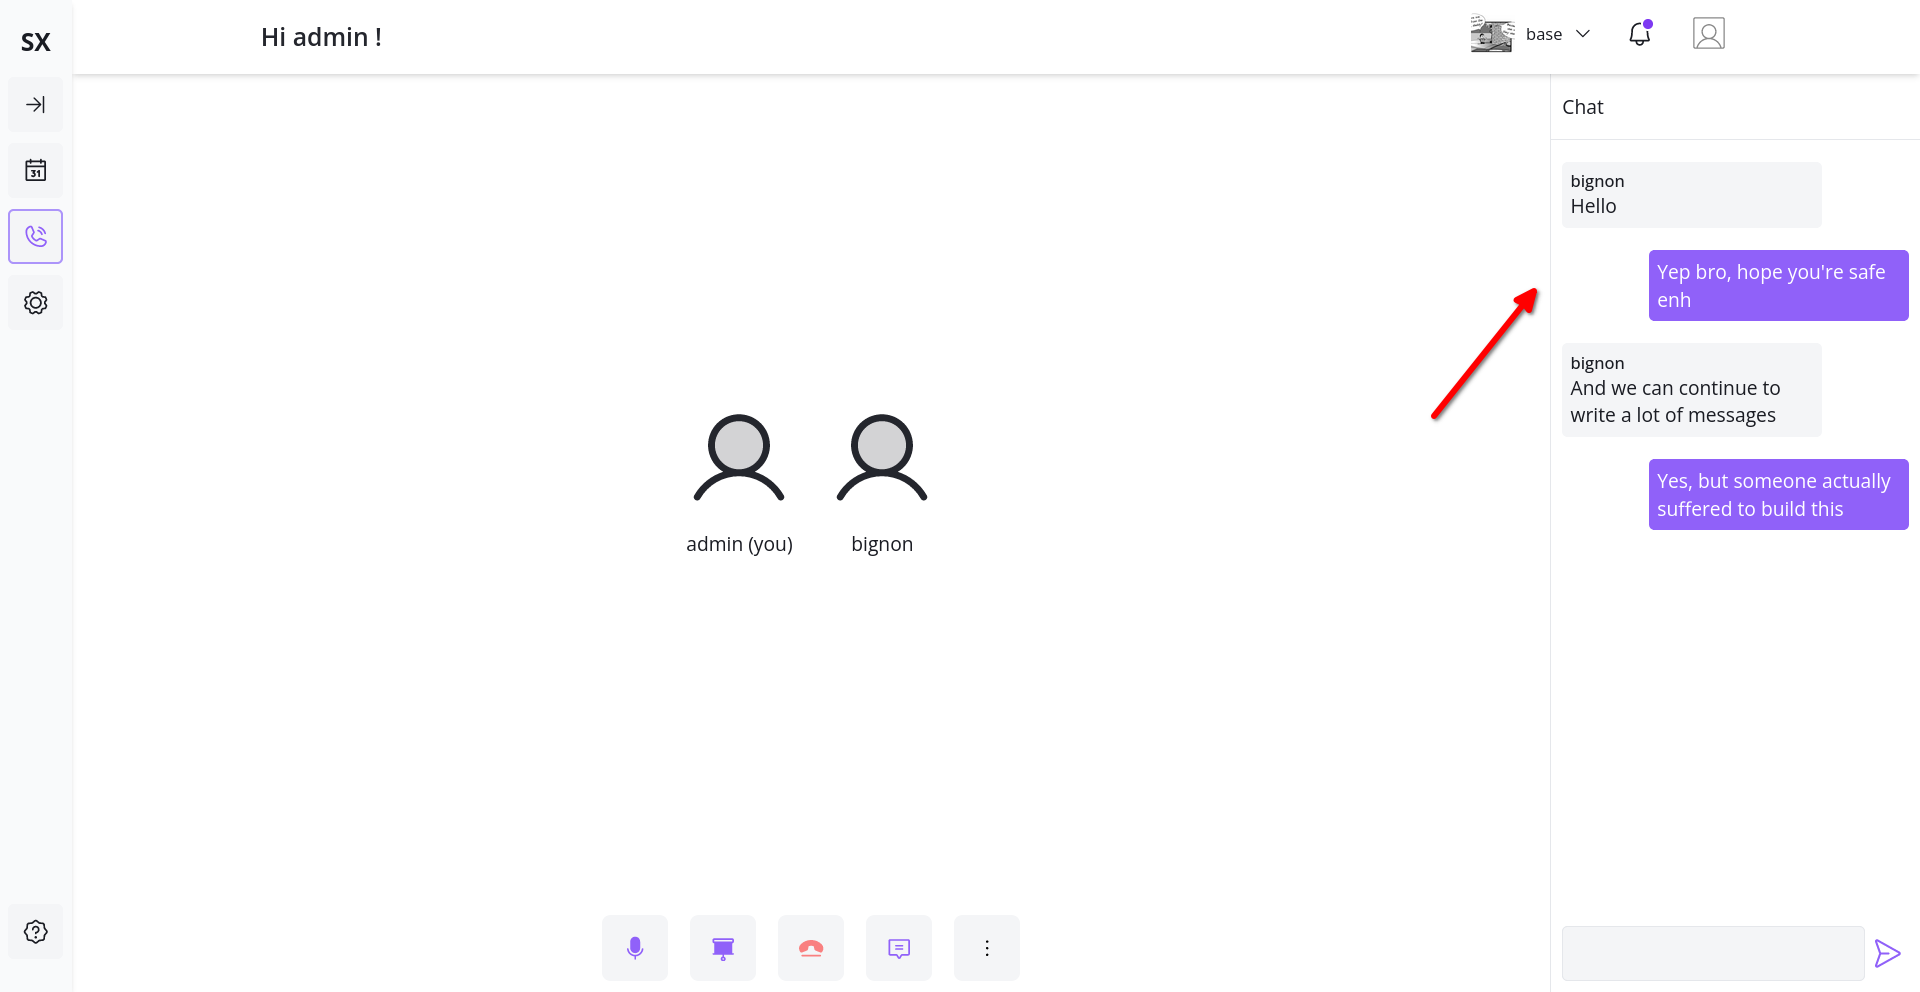
\includegraphics[width=0.85\textwidth]{prototype/room-chat}}
  \caption{Messagerie instantannée intégrée à \textbf{StudX}}
  \label{fig:room_chat}
\end{figure}

Plusieurs autres fonctionnalités sont exploitables. 
L’une d’elles est le partage d'écran. Pour illustrer, nous nous sommes servis de deux appareils avec 
l’un faisant le partage, comme le montre les figures \ref{fig:sharing_screen} et \ref{fig:viewing_screen}.

\newpage
\begin{figure}[h]
  \centering
  \frame{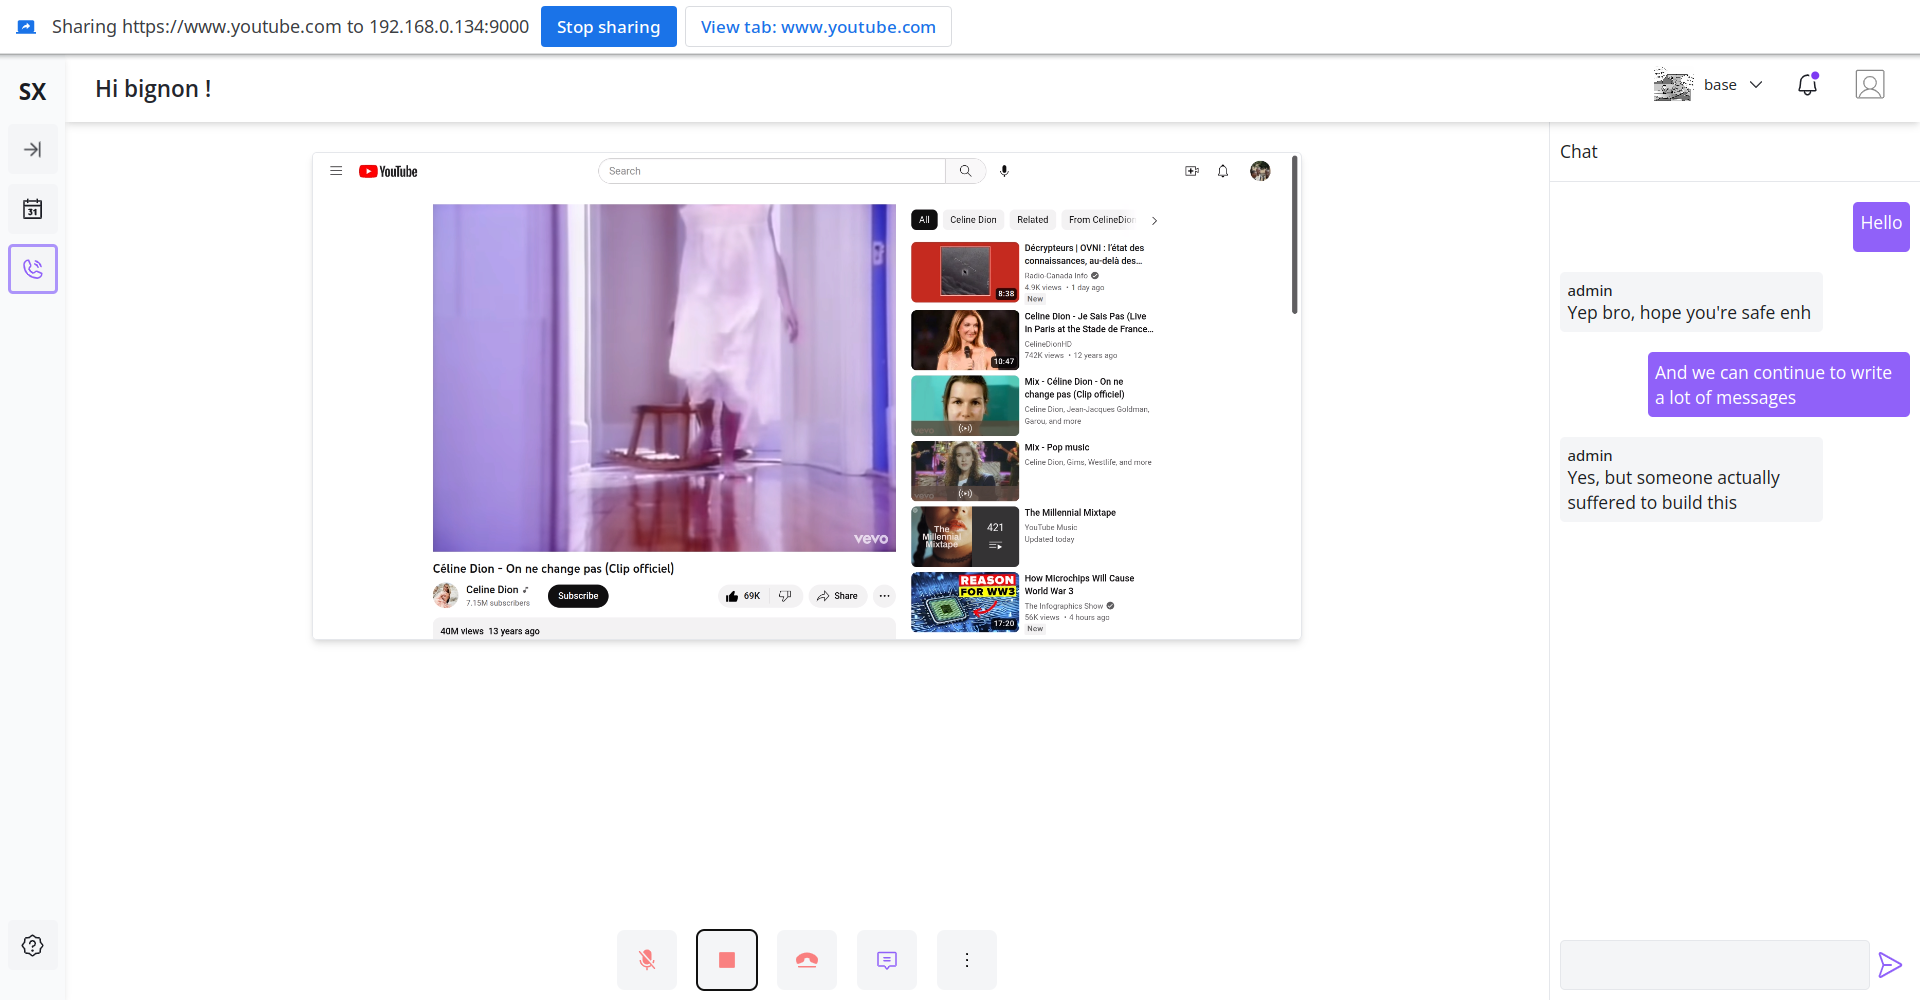
\includegraphics[width=0.85\textwidth]{prototype/user-sharing-screen}}
  \caption{Partage d'écran}
  \label{fig:sharing_screen}
\end{figure}

\newpage
\begin{figure}[h]
  \centering
  \frame{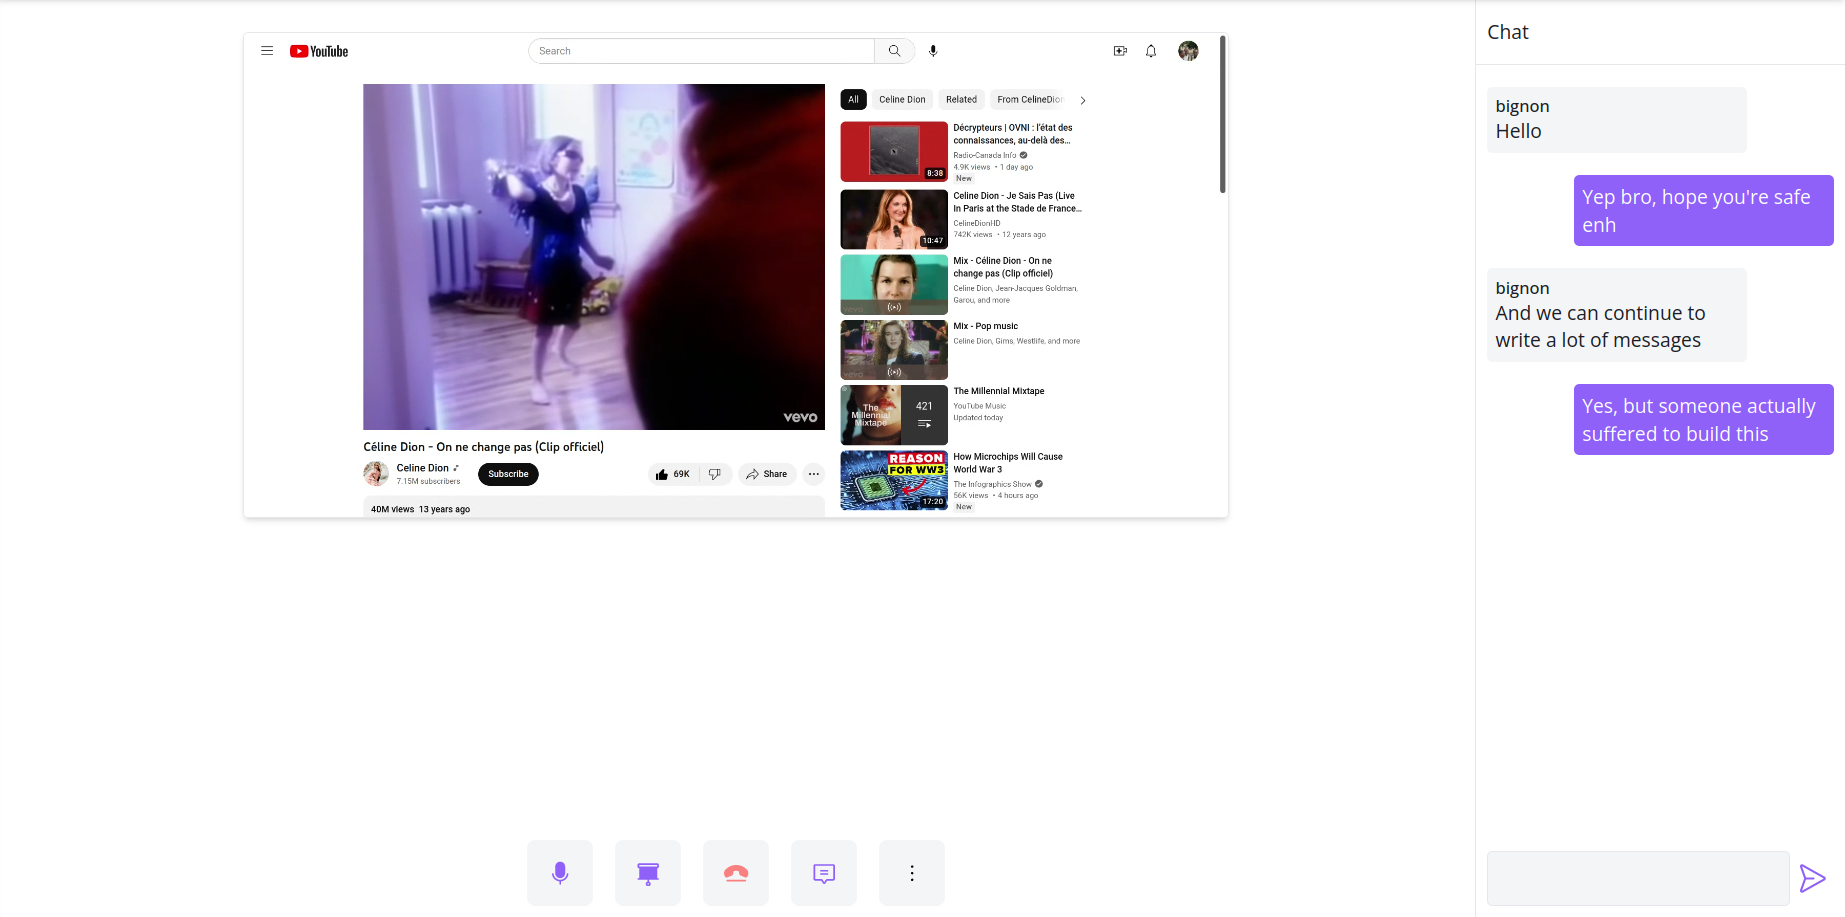
\includegraphics[width=0.85\textwidth]{prototype/user-viewing-screen}}
  \caption{Visualisation de l'écran partagé}
  \label{fig:viewing_screen}
\end{figure}

Les participants disposent également d’un whiteboard, 
c'est-à- dire un tableau virtuel, pour effectuer des illustrations. 
Le contenu est synchronisé entre tous les participants. 
La figure 3.10 fait une démonstration de ladite fonction.

\begin{figure}[h]
  \centering
  \frame{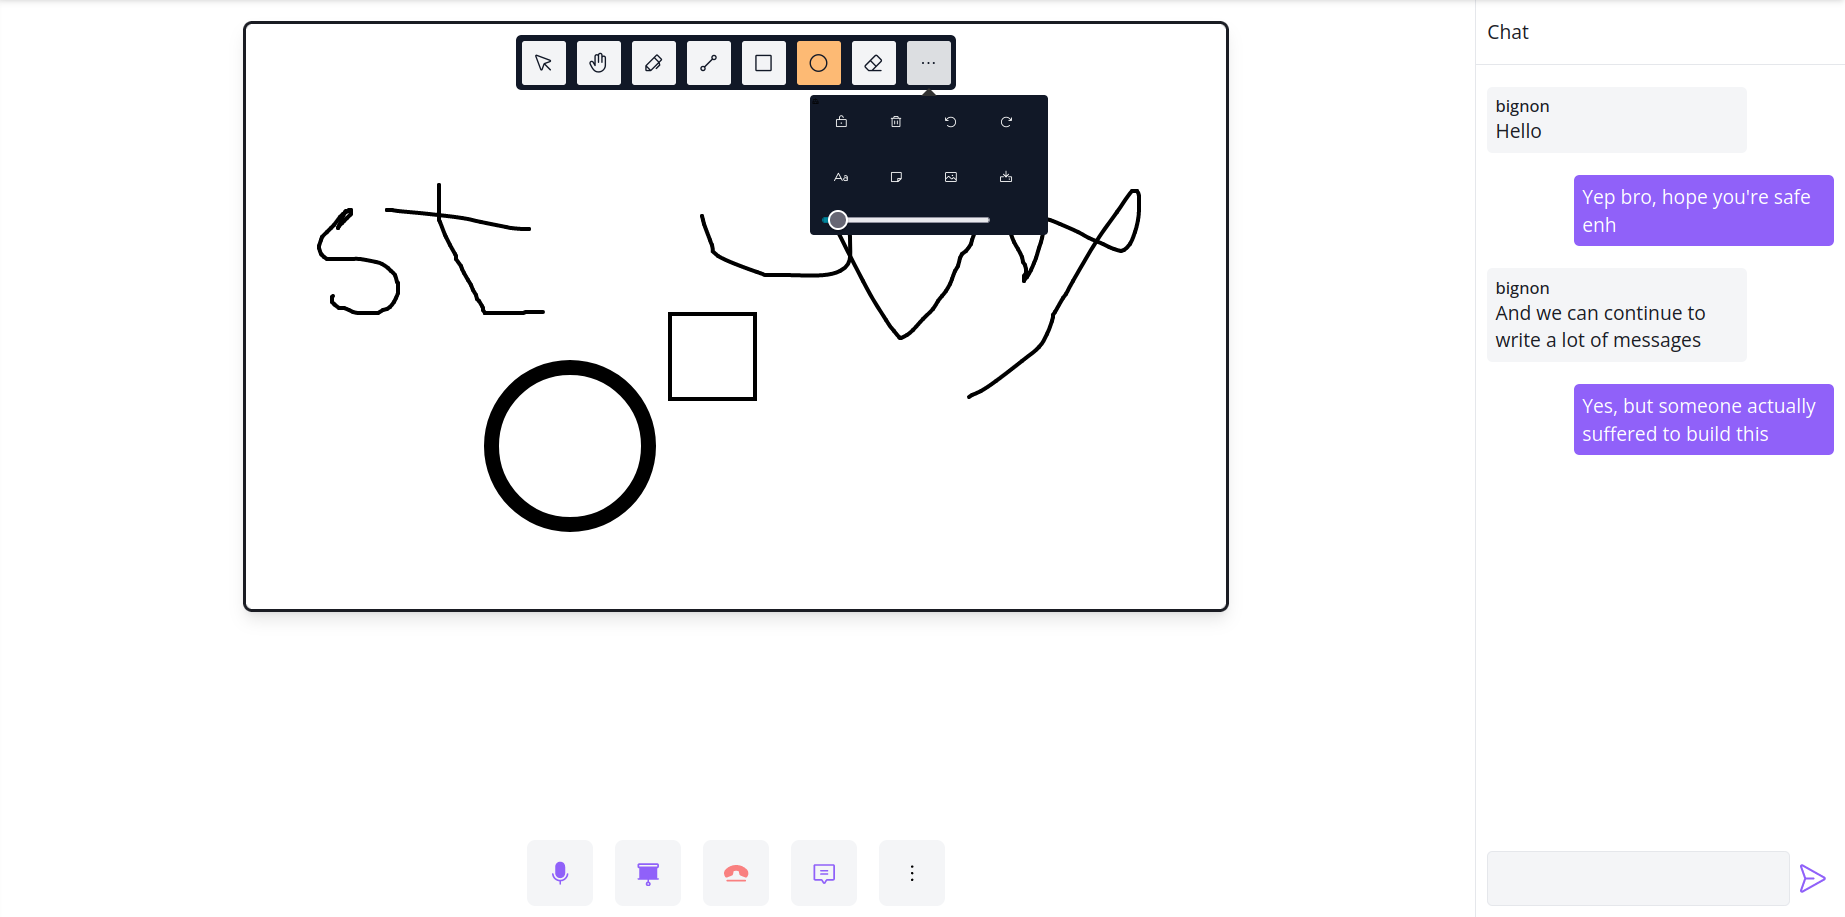
\includegraphics[width=0.85\textwidth]{prototype/whiteboard}}
  \caption{Tableau virtuel}
  \label{fig:whiteboard}
\end{figure}

On peut également percevoir sur l’image, les modifications apportées au projet Open Source qui a servi de base au développement de cette fonctionnalité.

L’application dispose également d’un dispositif de notes intégré, que nous qualifions de \textbf{Writepad}. La figure \ref{fig:writepad} la présente.


\begin{figure}[h]
  \centering
  \frame{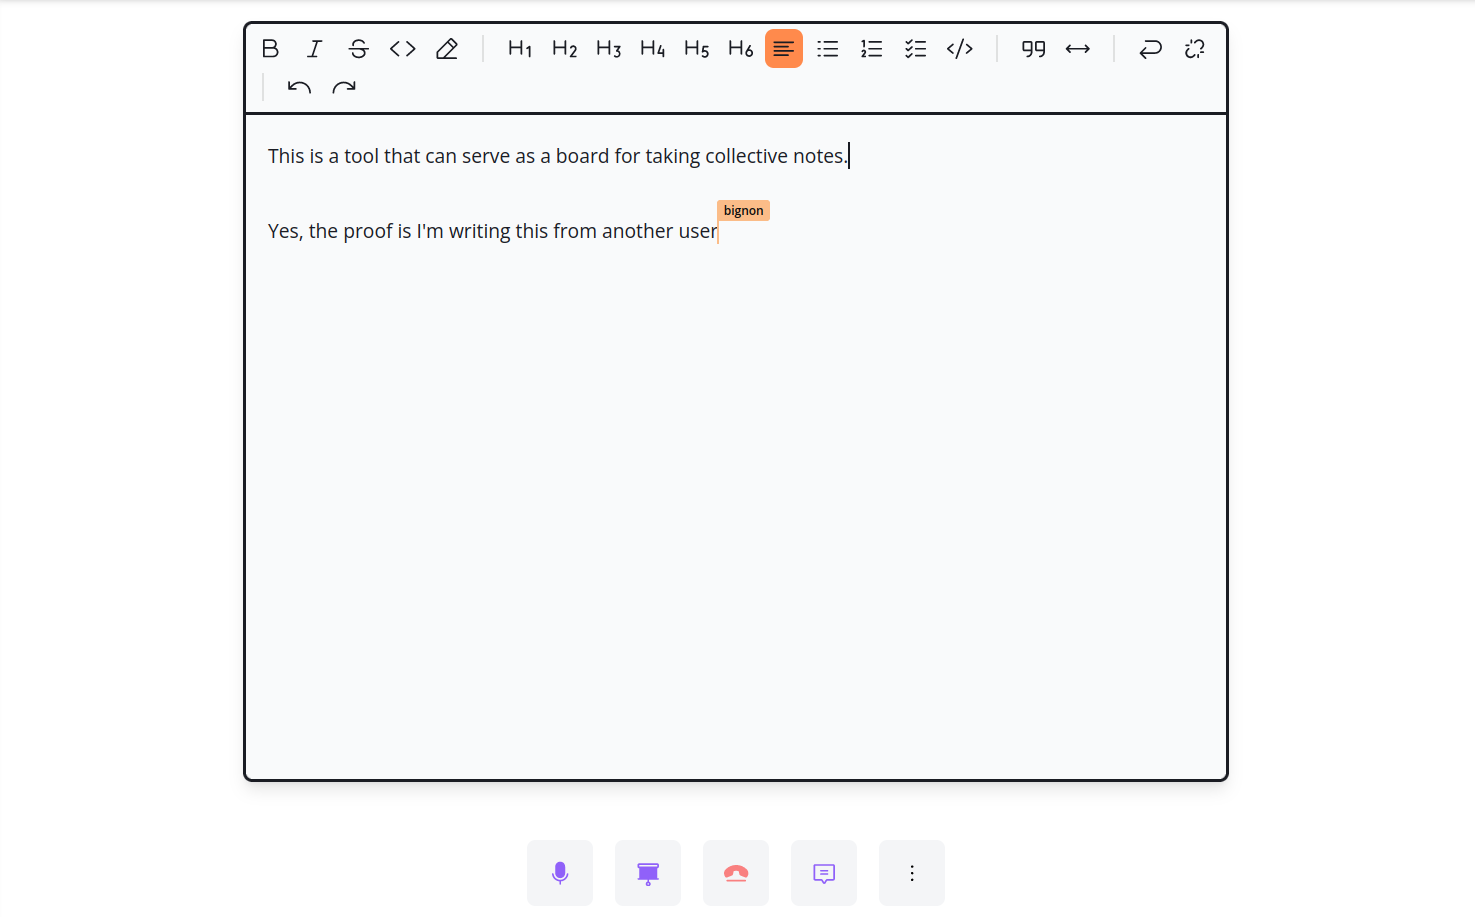
\includegraphics[width=0.85\textwidth]{prototype/wrritepad}}
  \caption{Outil de note synchronisé}
  \label{fig:writepad}
\end{figure}

Les fonctions suscitées rendent inaccessible la grille des participants. 
Mais il est toujours possible de pourvoir y accéder dans la même section que la messagerie, comme le montre la figure \ref{fig:participants_aside}.

\newpage
\begin{figure}[h]
  \centering
  \frame{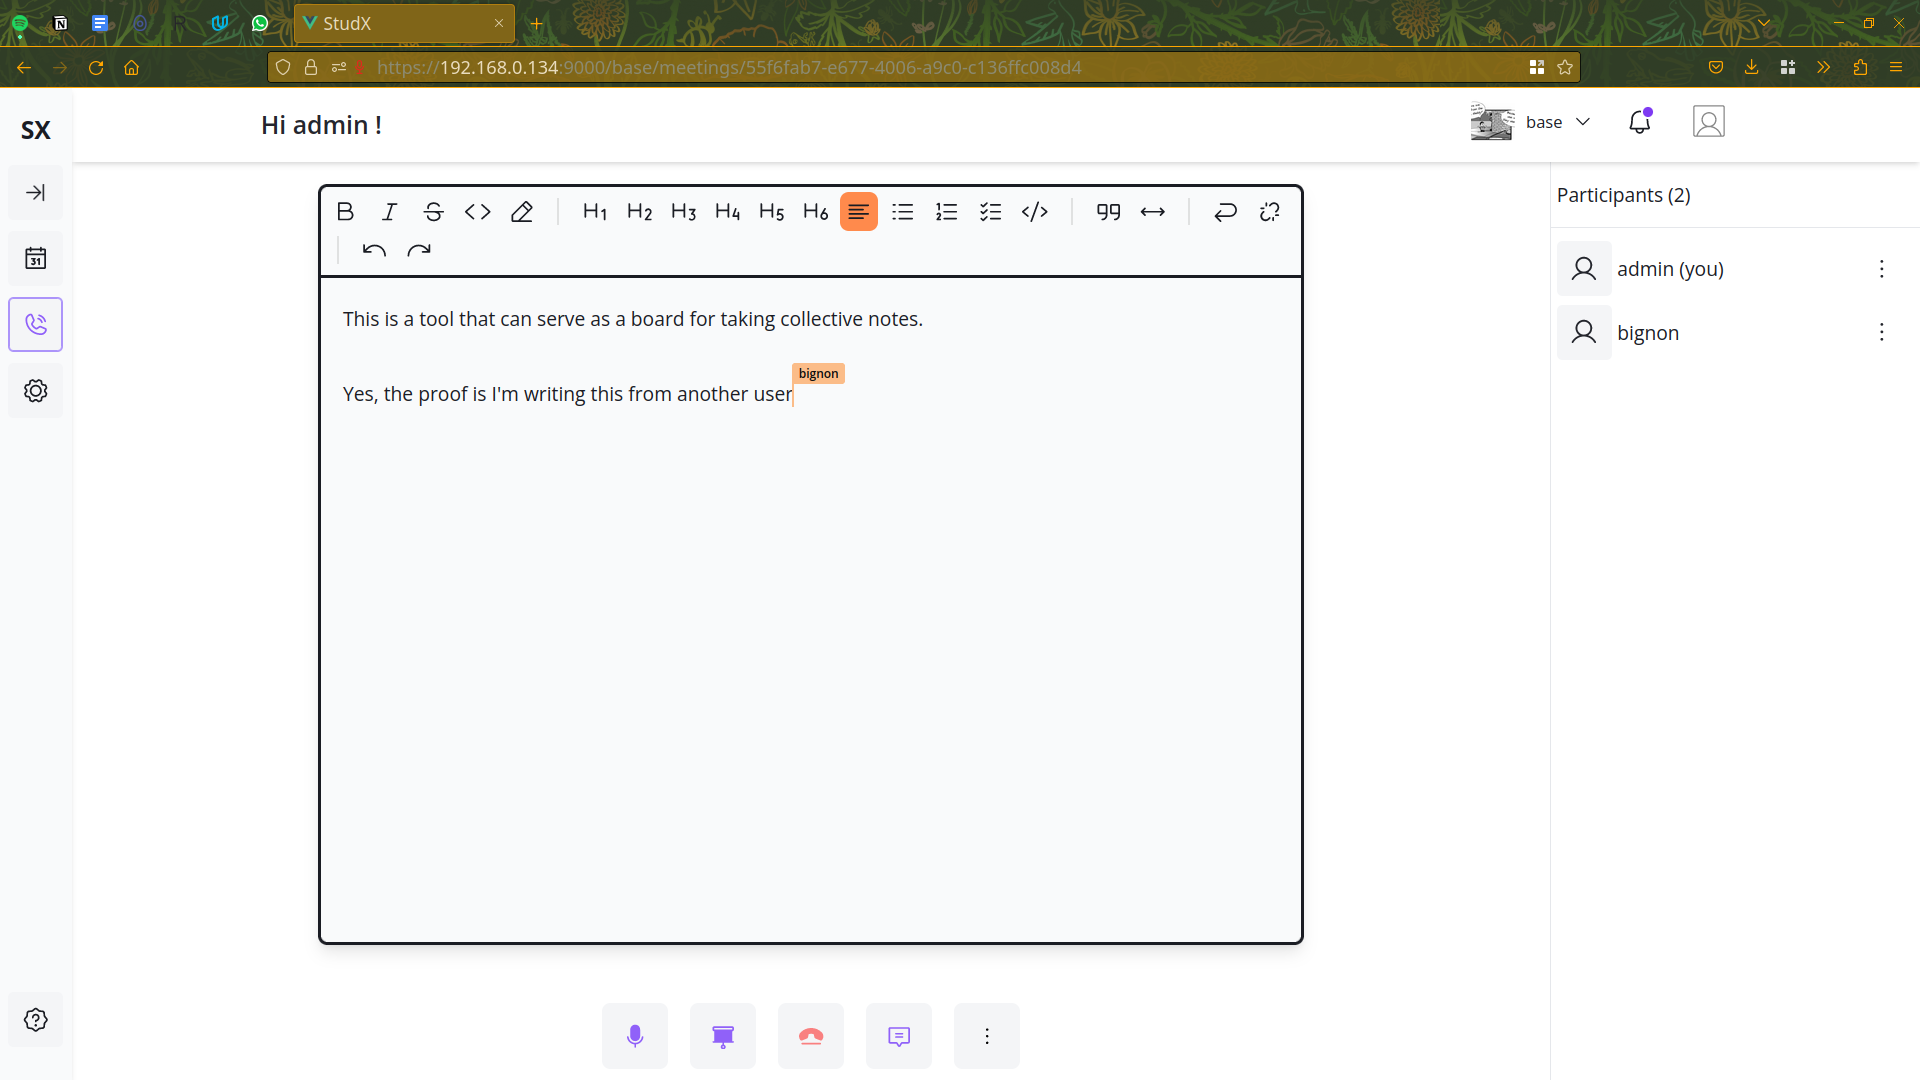
\includegraphics[width=0.85\textwidth]{prototype/participants}}
  \caption{Liste des participants}
  \label{fig:participants_aside}
\end{figure}

Enfin, chaque utilisateur a la possibilité de quitter la réunion. Si par mégarde, il essaie de recharger par exemple, l’onglet, une confirmation est requise (si le navigateur supporte cette fonctionnalité). 
Les figures \ref{fig:confirm_exit} et \ref{fig:exited} en font l'illustration.

\newpage
\begin{figure}[h]
  \centering
  \frame{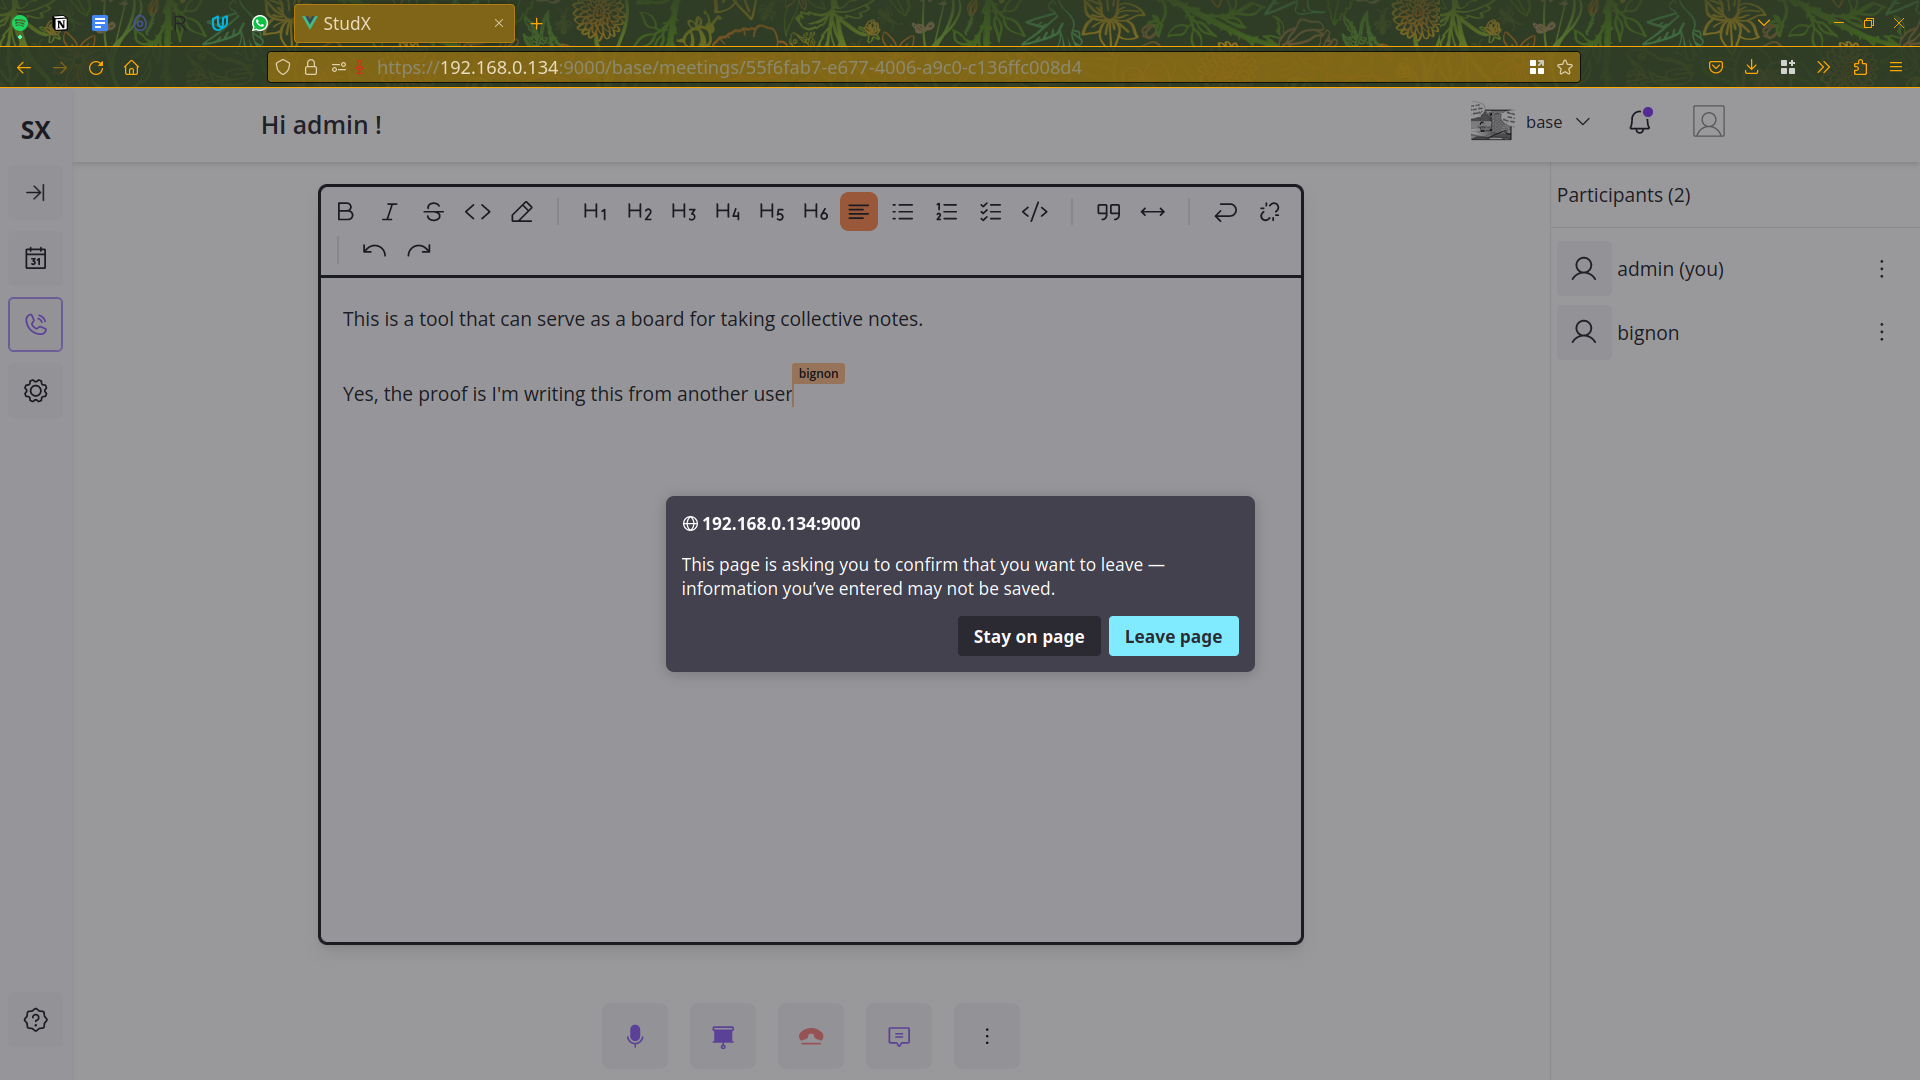
\includegraphics[width=0.85\textwidth]{prototype/confirm-exit}}
  \caption{Confirmation de déconnexion}
  \label{fig:confirm_exit}
\end{figure}

\begin{figure}[h]
  \centering
  \frame{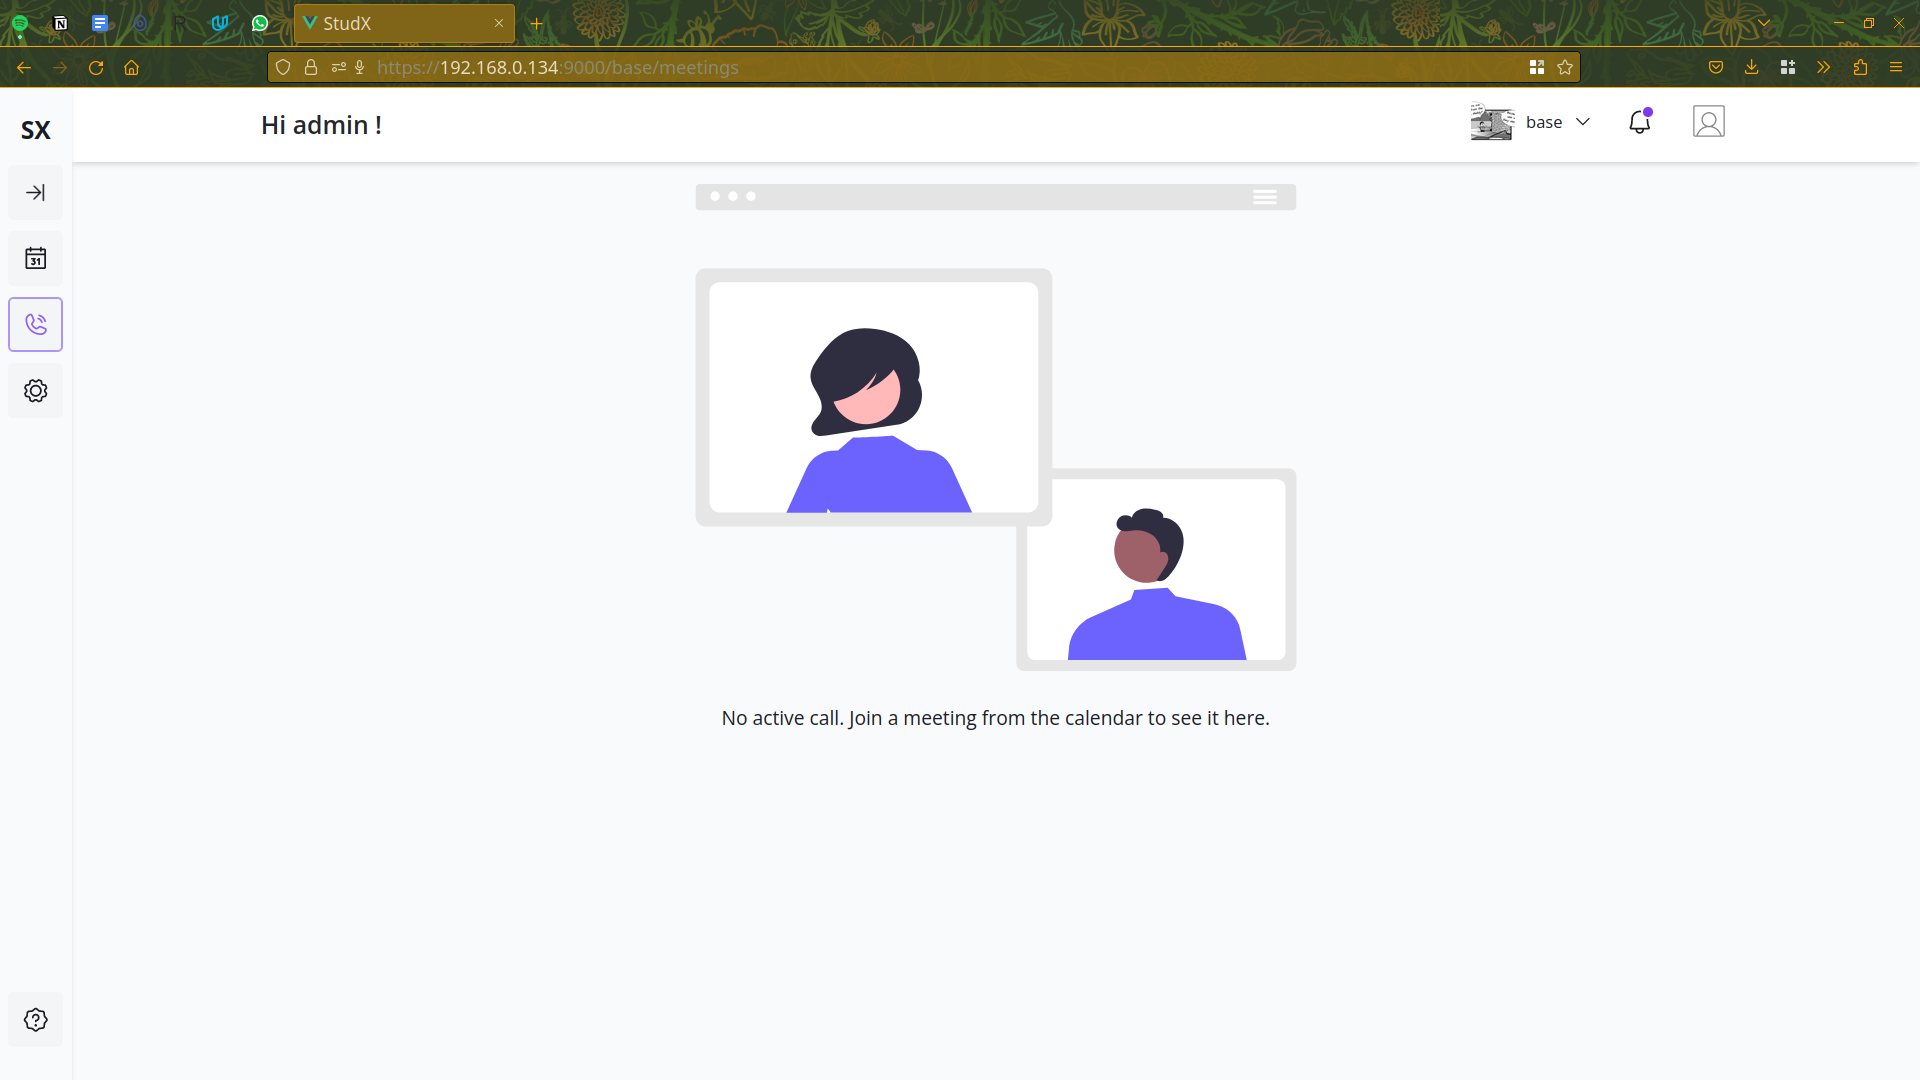
\includegraphics[width=0.85\textwidth]{prototype/no-active-call}}
  \caption{Page de redirection après déconnexion}
  \label{fig:exited}
\end{figure}

\subsection{Autres fonctionnalités}
Dans le but d'améliorer l'expérience utilisateur, nous avons jugé utile d’ajouter quelques fonctionnalités outre celles initialement visées. 
Parmi elles figurent le mode sombre et la mise en place d’un tutoriel interactif expliquant les diverses composantes de notre application. 

\newpage
\begin{figure}[h]
  \centering
  \frame{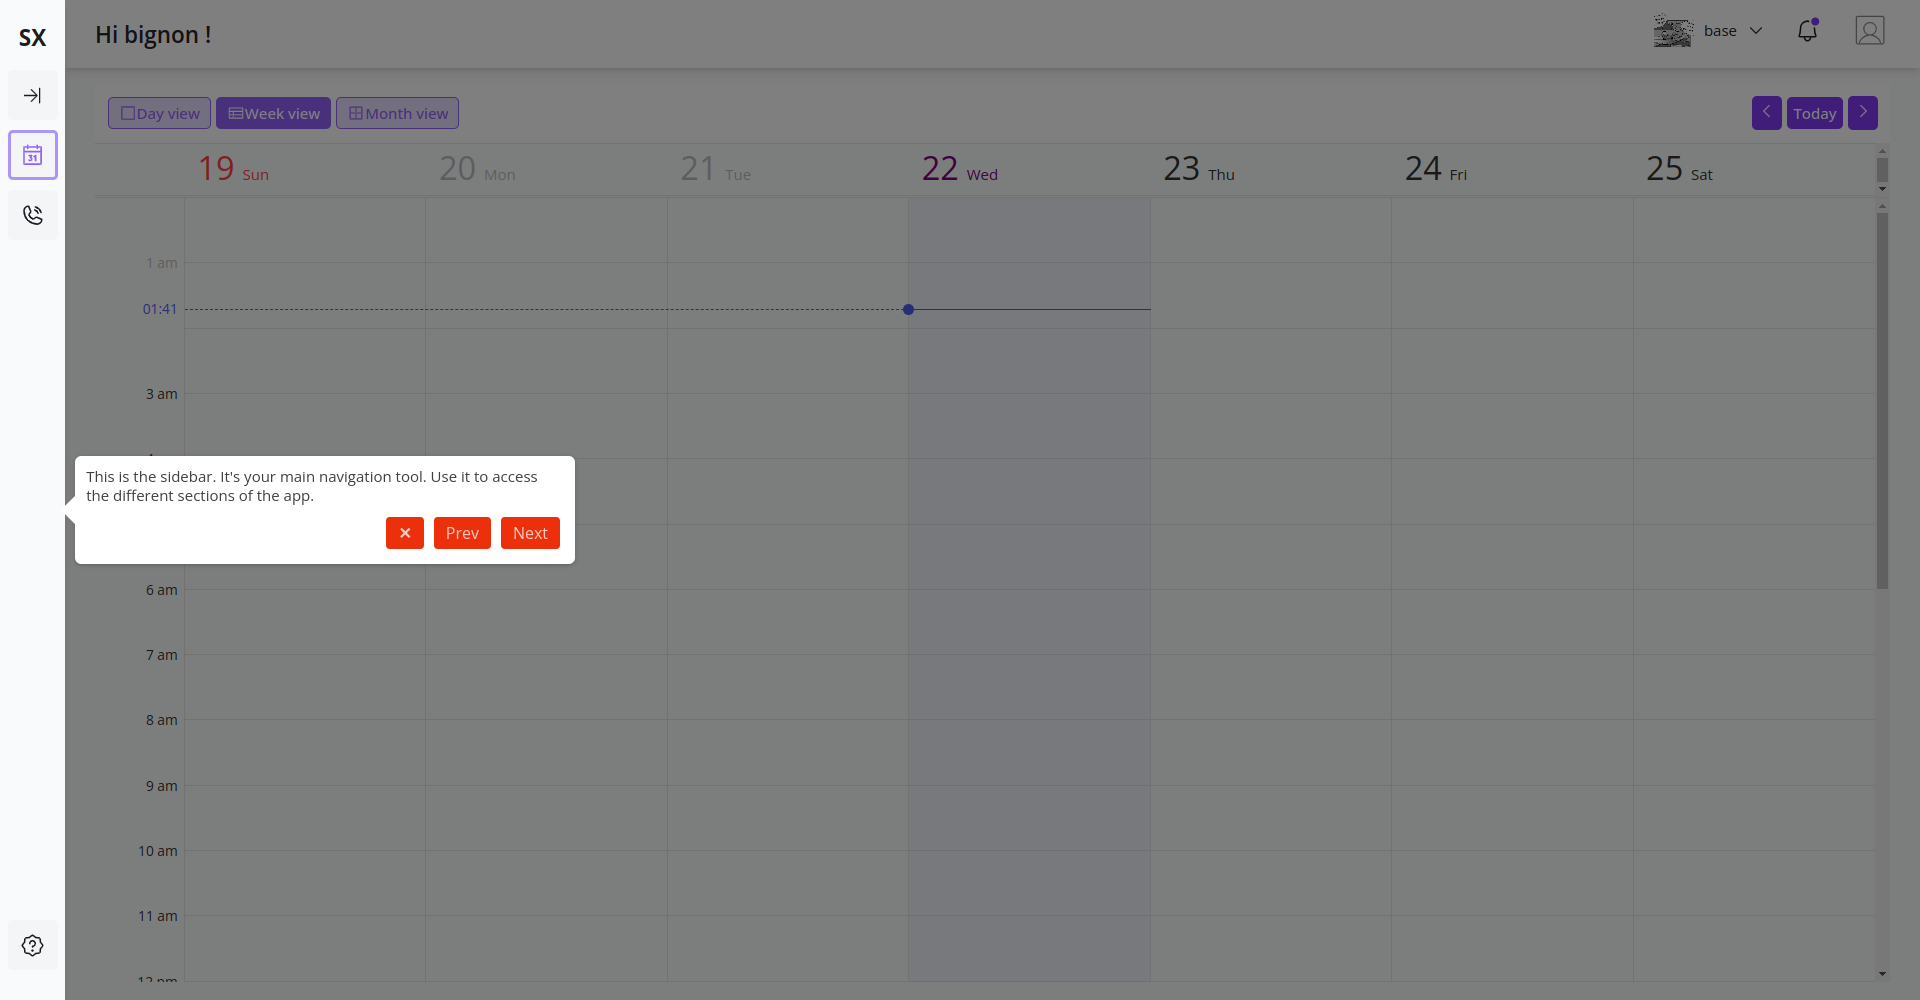
\includegraphics[width=0.85\textwidth]{prototype/user-onboarding}}
  \caption{Tutoriel interactif d’introduction à StudX}
  \label{fig:onboarding}
\end{figure}


\begin{figure}[h]
  \centering
  \frame{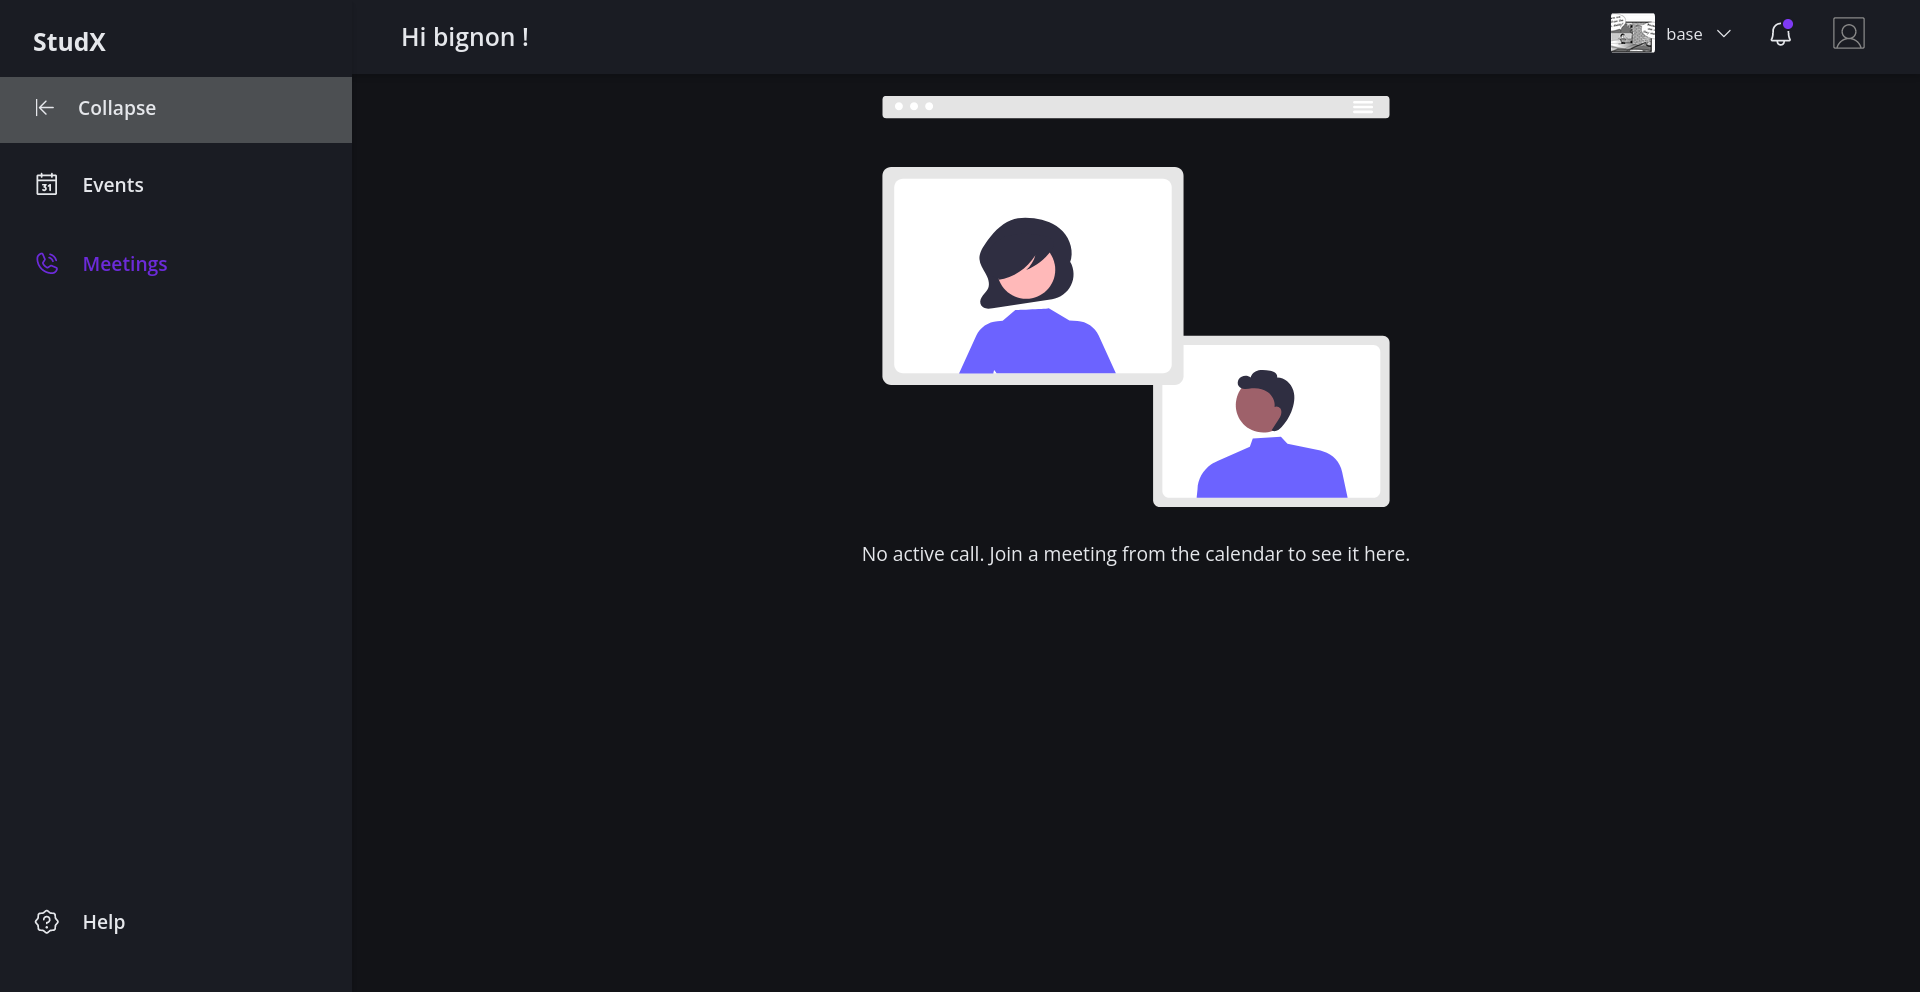
\includegraphics[width=0.85\textwidth]{prototype/wip-dark-mode}}
  \caption{Mode sombre}
  \label{fig:dark_mode}
\end{figure}

Les administrateurs de la plateforme disposent également d’un accès aux paramètres de 
l'organisation qu’ils dirigent et peuvent ainsi ajouter ou retirer des membres (figures \ref{fig:settings_one} et \ref{fig:settings_two}).

\begin{figure}[h]
  \centering
  \frame{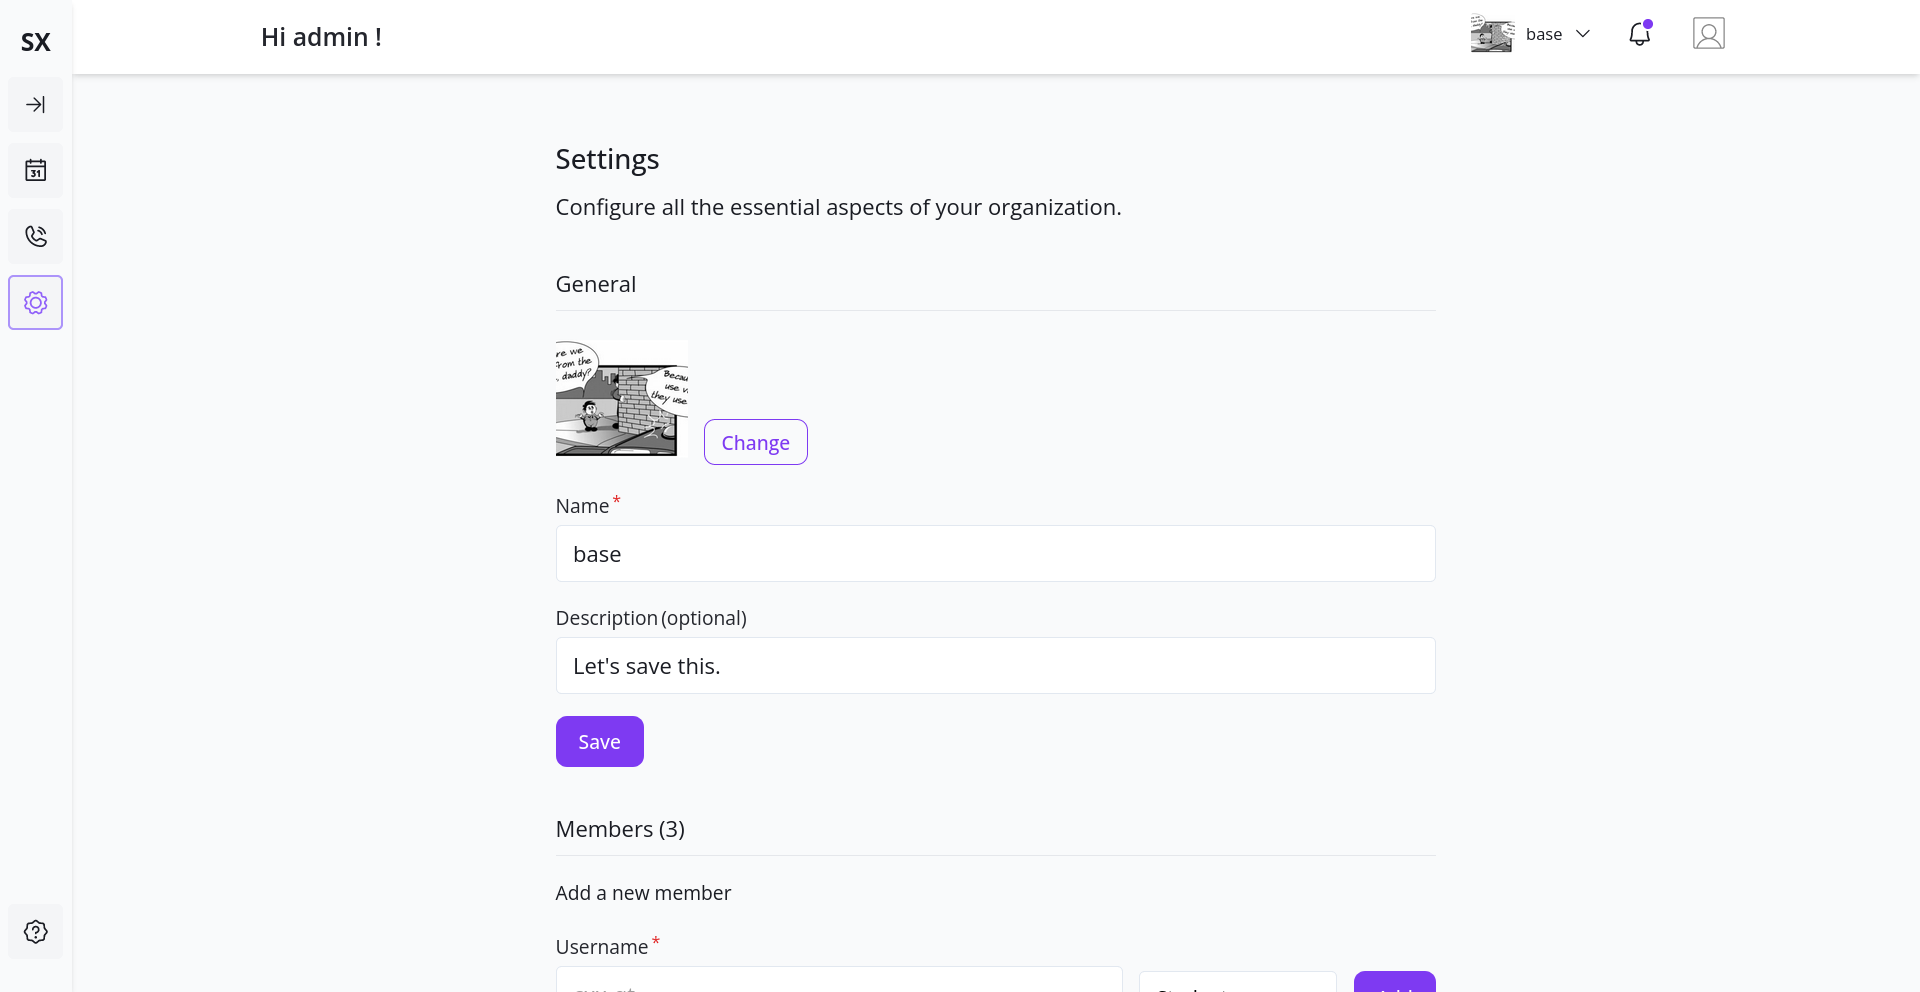
\includegraphics[width=0.85\textwidth]{prototype/settings}}
  \caption{Mode sombre}
  \label{fig:settings_one}
\end{figure}

\begin{figure}[h]
  \centering
  \frame{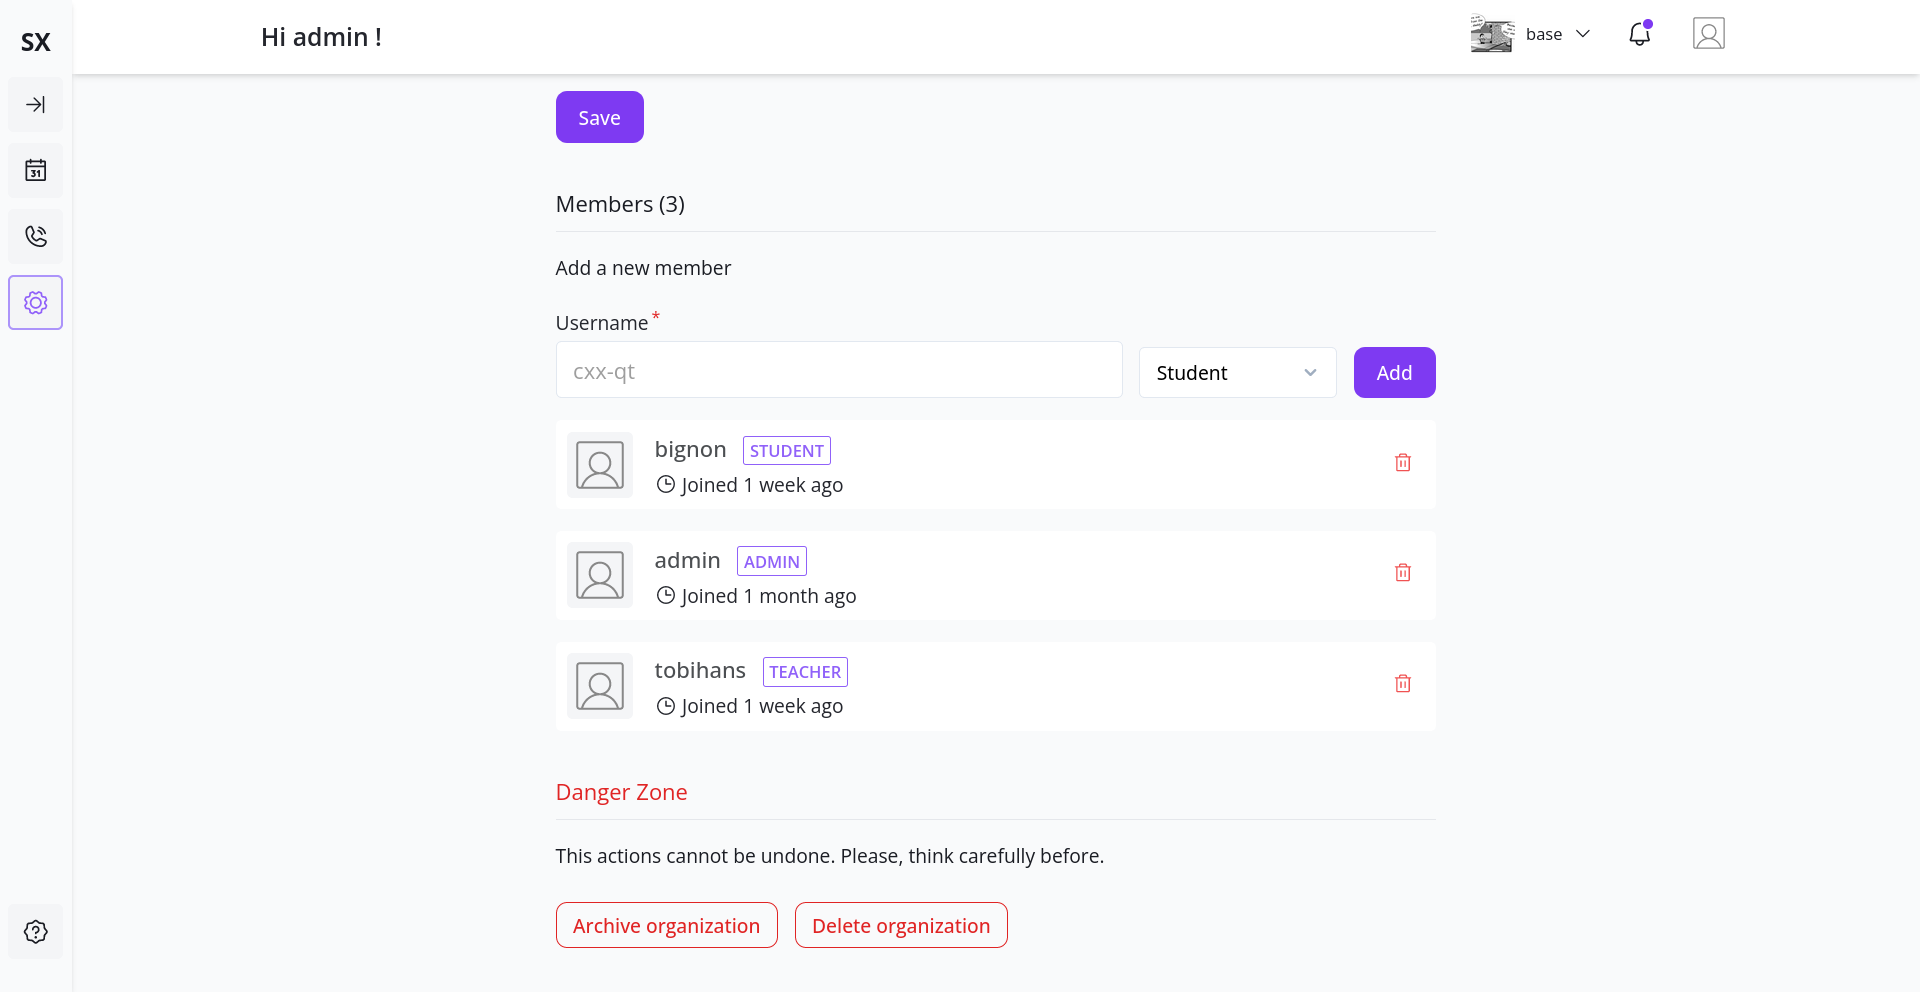
\includegraphics[width=0.85\textwidth]{prototype/settings-end}}
  \caption{Mode sombre}
  \label{fig:settings_two}
\end{figure}

\newpage
\section{Perspectives}
Le prototype StudX présente un ensemble de fonctionnalités utiles pour le déroulement de classes virtuelles. 
Toutefois, il présente certaines limites, outre les choix de conception comme l’absence de flux vidéo. 

En effet, la plateforme est conçue pour être accessible aux personnes disposant de toutes leurs facultés. 
Bien que les règles basiques d'accessibilité soient prises en compte, 
elles ne couvrent pas totalement le besoin. Par exemple, les personnes malentendantes 
n’ont pas la capacité de tirer profit des échanges vocaux qui sont effectués entre les divers participants. 
Une fonctionnalité envisagée est l'intégration de modèle de Machine Learning permettant la conversion de 
ces signaux audio en gestuelles dans le langage sourd.

Par ailleurs, dans le cadre d’un prototype, les fonctionnalités sont plutôt restreintes. 
On peut ajouter ou améliorer des fonctions comme la persistance de la messagerie instantanée ou 
encore la gestion des utilisateurs.


\addcontentsline{toc}{section}{Conclusion}
\section*{Conclusion}
Le prototype conçu répond à bien des besoins et couvre un tant soit peu l’ensemble des objectifs visés. 
Toutefois, il est possible de l’améliorer, dans le but d’en faire un plus large usage.

% \include{perspectives}
%%conclusion
\conclusion
Bla bla bla \cite{ehrig2006graph}
% 
% \lhead[]{} \rhead[]{} \chead[]{}

%%biblio

%\chapter*{Annexe}\addcontentsline{toc}{chapter}{Annexe}\label{annexe1}

\subsection*{Étapes clés du déroulement de l'attaque}


Nous allons exploiter quelques failles de ce réseau pour effectuer une attaque man in the middle (MITM).\\

Au début, notre machine Windows peut atteindre normalement le routeur R4.
\begin{figure}[H]
    \centering
    \includegraphics[scale=0.8]{images/ping_b4_1}
    \caption{Ping vers le routeur R4 avec succès}
    \label{fig:ping_b4_1}
\end{figure}
Quand on essaie de tracer le chemin vers R4, on constate que la machine passe par le routeur R1 légitime du lien pour atteindre R4
\begin{figure}[H]
    \centering
    \includegraphics{images/tracert_b4_1}
    \caption{Traces du chemin vers R4}
    \label{fig:tracert_b41}
\end{figure}
L'attaquant sur le lien peut alors passer a l'attaque.
Pour effectuer l'attaque MITM on utilisera l'outil fake\_router6, un utilitaire du package d'outils \textbf{the hacker choice}.
Ainsi sur la machine d'attaque, on active en un premier lieu le forwarding pour être transparent et ne pas bloquer le transit des paquets.
\begin{figure}[H]
    \centering
    \includegraphics{images/attk/fwrd_activation}
    \caption{Activation du forwarding des paquets.}
    \label{fig:activ_fwrd}
\end{figure}
Aussi on lance wireshark pour observer le trafic des paquets sur notre interface dans le réseau.\\
-------\\
Puisque tout est prêt nous allons lancer l'attaque.

\begin{figure}[H]
    \centering
    \includegraphics[scale=0.8]{images/attk/lancement_attk_1}
    \caption{Initialisation de l'attaque}
    \label{fig:attk_init_1}
\end{figure}

L'attaque est en cours et l'attaquant s'annonce comme le routeur par défaut du lien
nous allons maintenant vérifier la table des routes de notre machine windows.
\begin{figure}[H]
    \centering
    \includegraphics{images/attk/tableRoutes_windows}
    \caption{Table des routes de la machine victime}
    \label{fig:win_route_table}
\end{figure}
On constate que l'attaquant s'est insère comme passerelle de la victime.
pour confirmer cela reprenons un tracert vers le routeur r4
\begin{figure}[H]
    \centering
    \includegraphics{images/attk/tracert_b4_2}
    \caption{Chemin vers b4 pendant l'attaque.}
    \label{fig:tracert_b42}
\end{figure}
On peut voir clairement que la victime passe par l'attaquant pour atteindre le routeur.\\

A présent nous allons essayer de capturer une information envoyée par la victime.
Pour cela la victime fait un telnet sur le router R4 pour s'y connecter avec les paramètres suivants:\\
password1:\textbf{cisco}\\
password2:\textbf{class}
\begin{figure}[H]
    \centering
    \includegraphics{images/attk/telnet_r4}
    \caption{Connexion telnet au routeur.}
    \label{fig:telnetr4}
\end{figure}

Une fois la connexion réussie, nous allons voir avec wireshark les paquets de connexion et y retrouver les paramètres de connexion.
\begin{figure}[H]
    \centering
    \includegraphics[width=1.0\textwidth]{images/attk/c}
    \includegraphics[width=1.0\textwidth]{images/attk/i}
    \includegraphics[width=1.0\textwidth]{images/attk/s}
    \includegraphics[width=1.0\textwidth]{images/attk/c2}
    \includegraphics[width=1.0\textwidth]{images/attk/o}   
    \caption{Premier paramètre de connexion au routeur R4: \textbf{c-i-s-c-o}}
    \label{fig:param_conn_r4}
\end{figure}
\begin{figure}[H]
    \centering
    \includegraphics[width=1.0\textwidth]{images/attk/param2_c}
    \includegraphics[width=1.0\textwidth]{images/attk/param2_l}
    \includegraphics[width=1.0\textwidth]{images/attk/param2_a}
    \includegraphics[width=1.0\textwidth]{images/attk/param2_s1}
    \includegraphics[width=1.0\textwidth]{images/attk/param2_s2}
    \caption{Second paramètre de connexion au routeur R4: \textbf{c-l-a-s-s}}
    \label{fig:param_conn2}
\end{figure}
Les paramètres on été retrouves donc l'attaque a été un succès!

%\subsection*{Mitigations}
%Pour sécuriser ce réseau afin d'éviter ce genre d'attaque, deux mesures de sécurité peuvent être configurées.
%\begin{itemize}
%    \item le SEND
%    \item le RaGuard
%\end{itemize}



\end{document}
